\documentclass{beamer}
%
% Choose how your presentation looks.
%
% For more themes, color themes and font themes, see:
% http://deic.uab.es/~iblanes/beamer_gallery/index_by_theme.html
%
\mode<presentation>
{
  \usetheme{default}      % or try Darmstadt, Madrid, Warsaw, ...
  \usecolortheme{default} % or try albatross, beaver, crane, ...
  \usefonttheme{default}  % or try serif, structurebold, ...
  \setbeamertemplate{navigation symbols}{}
  \setbeamertemplate{caption}[numbered]
} 
% CUSTOM
\makeatletter
\newcommand*{\rom}[1]{\expandafter\@slowromancap\romannumeral #1@}


\makeatother

\usepackage[english]{babel}
\usepackage[utf8]{inputenc}
\usepackage[T1]{fontenc}
\usepackage{amsmath}
\usetheme{Antibes}
\usepackage{centernot}
\title[]{Introductory Course: Machine Learning (WWI15B4)}
\subtitle{Classification \rom{2}}
\author{Fabio Ferreira, David Bethge}
\institute{DHBW Karlsruhe}
\date{}
\graphicspath{{figures/04/}}

\DeclareMathOperator*{\argmax}{argmax}
\expandafter\def\expandafter\insertshorttitle\expandafter{%
   \insertshorttitle\hfill%
   \insertframenumber\,/\,\inserttotalframenumber}
   
   
\AtBeginSubsection[]
{
  \begin{frame}
    \frametitle{Table of Contents}
    \tableofcontents[currentsection,currentsubsection]
  \end{frame}
}


\begin{document}
%%%---CUSTOM---
%\bibliographystyle{plain}
%\bibliography{lecture/bibliography.bib}

\begin{frame}
  \titlepage
\end{frame}

\setbeamertemplate{caption}{\raggedright\insertcaption\par}


\section{Classification II}
\begin{frame}{Overview}
\tableofcontents
\end{frame}

\subsection{Introduction}
\begin{frame}{Recommended Literature}
\begin{center}
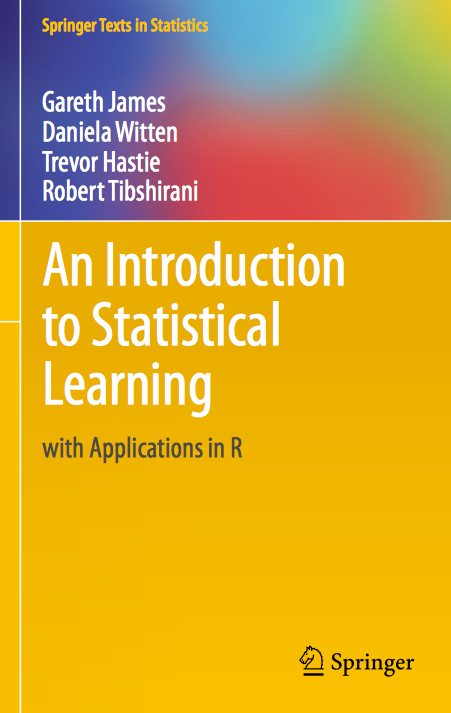
\includegraphics[width=0.3\textwidth]{classification_book}
\end{center}
or Stanford's CS231n course on CNNs is available online and gives a good introduction to classification and learning in computer vision
\end{frame}

\begin{frame}{Example}
\begin{figure}
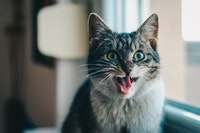
\includegraphics[width=0.2\textwidth]{cat}
\caption{cat image \emph{x}, shape [100x70x3]} 
\end{figure}


\begin{itemize}
\item parameter vector \emph{W}
\item $f(x,W) \longrightarrow$ 10 values indicating the class scores
\item ideally, the scalar representing 'cat' has highest value
\item W is a parameter vector used in \emph{parametric} function
\end{itemize}
\end{frame}

\begin{frame}{Parametric vs. Non-Parametric}
many definitions, among one is:
\begin{itemize}
\item \textbf{parametric}: model summarizes data by finite set of parameters, e.g. $$y_i=\boxed{\phi_0 + \phi_1x_i} + e_i$$
\item \textbf{non-parametric}: model (user) doesn't make explicit assumptions about the data distribution, e.g. $$y_i = \boxed{f(x_i)} + e_i$$
\item note: non-parametric methods still require parameters (however, their form isn't defined by the user)
\end{itemize}
\textbf{Task:} Classify the following ML approaches (parametric/non-parametric):
\begin{itemize}
\item decision tree
\item nearest neighbor
\item linear regression
\end{itemize}
\end{frame}


\subsection{Logistic Regression}

\begin{frame}{Example:Boston House Price dataset}
[The Boston house-price data of Harrison, D. and Rubinfeld, D.L. 'Hedonic
prices and the demand for clean air']
\begin{center}
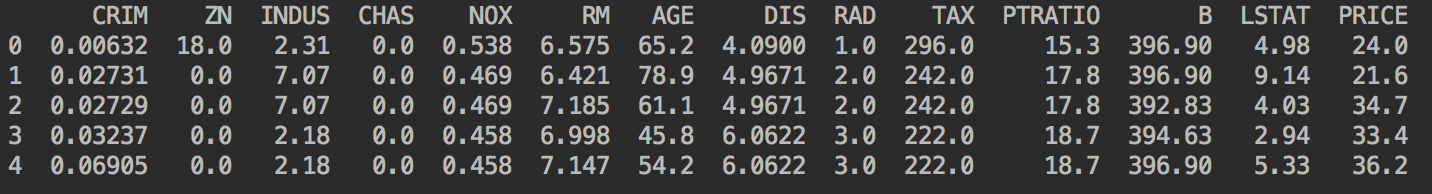
\includegraphics[width=1\textwidth]{boston}\\
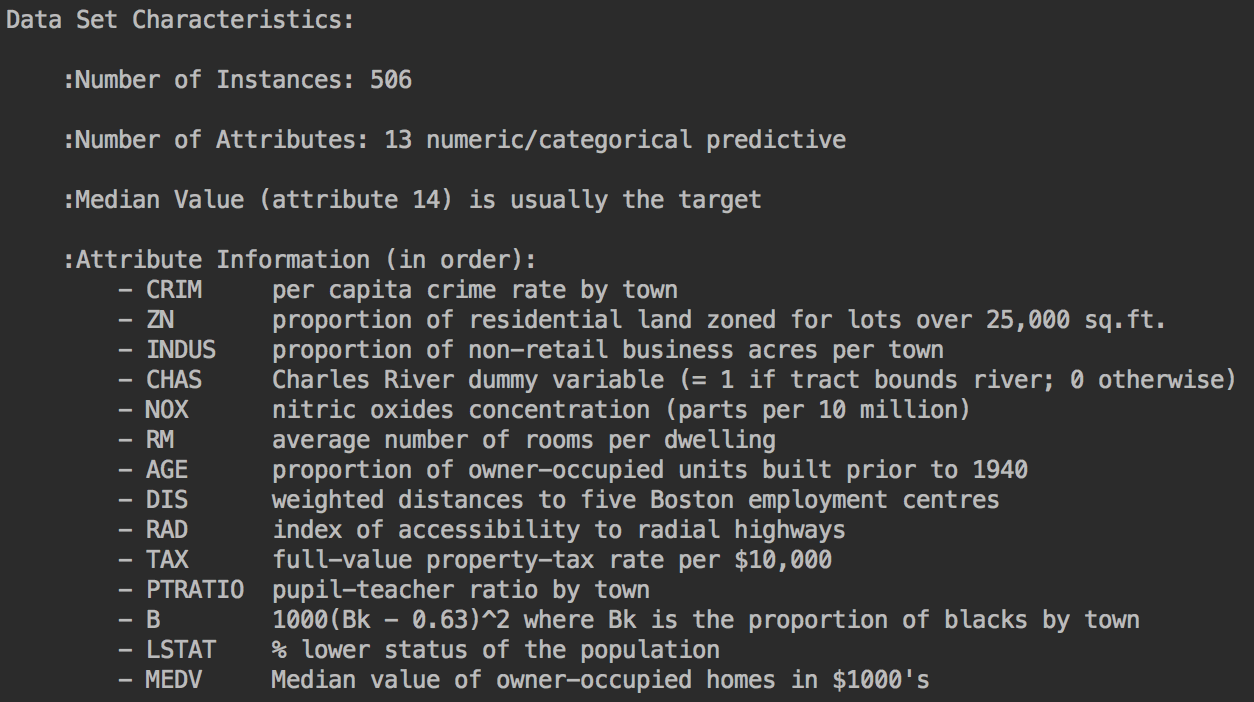
\includegraphics[width=0.7\textwidth, trim=0 9cm 0 0cm]{boston_descr}
\end{center}
\end{frame}

\begin{frame}{Boston House Price dataset}
Boston House Price covariance matrix\\
\begin{center}
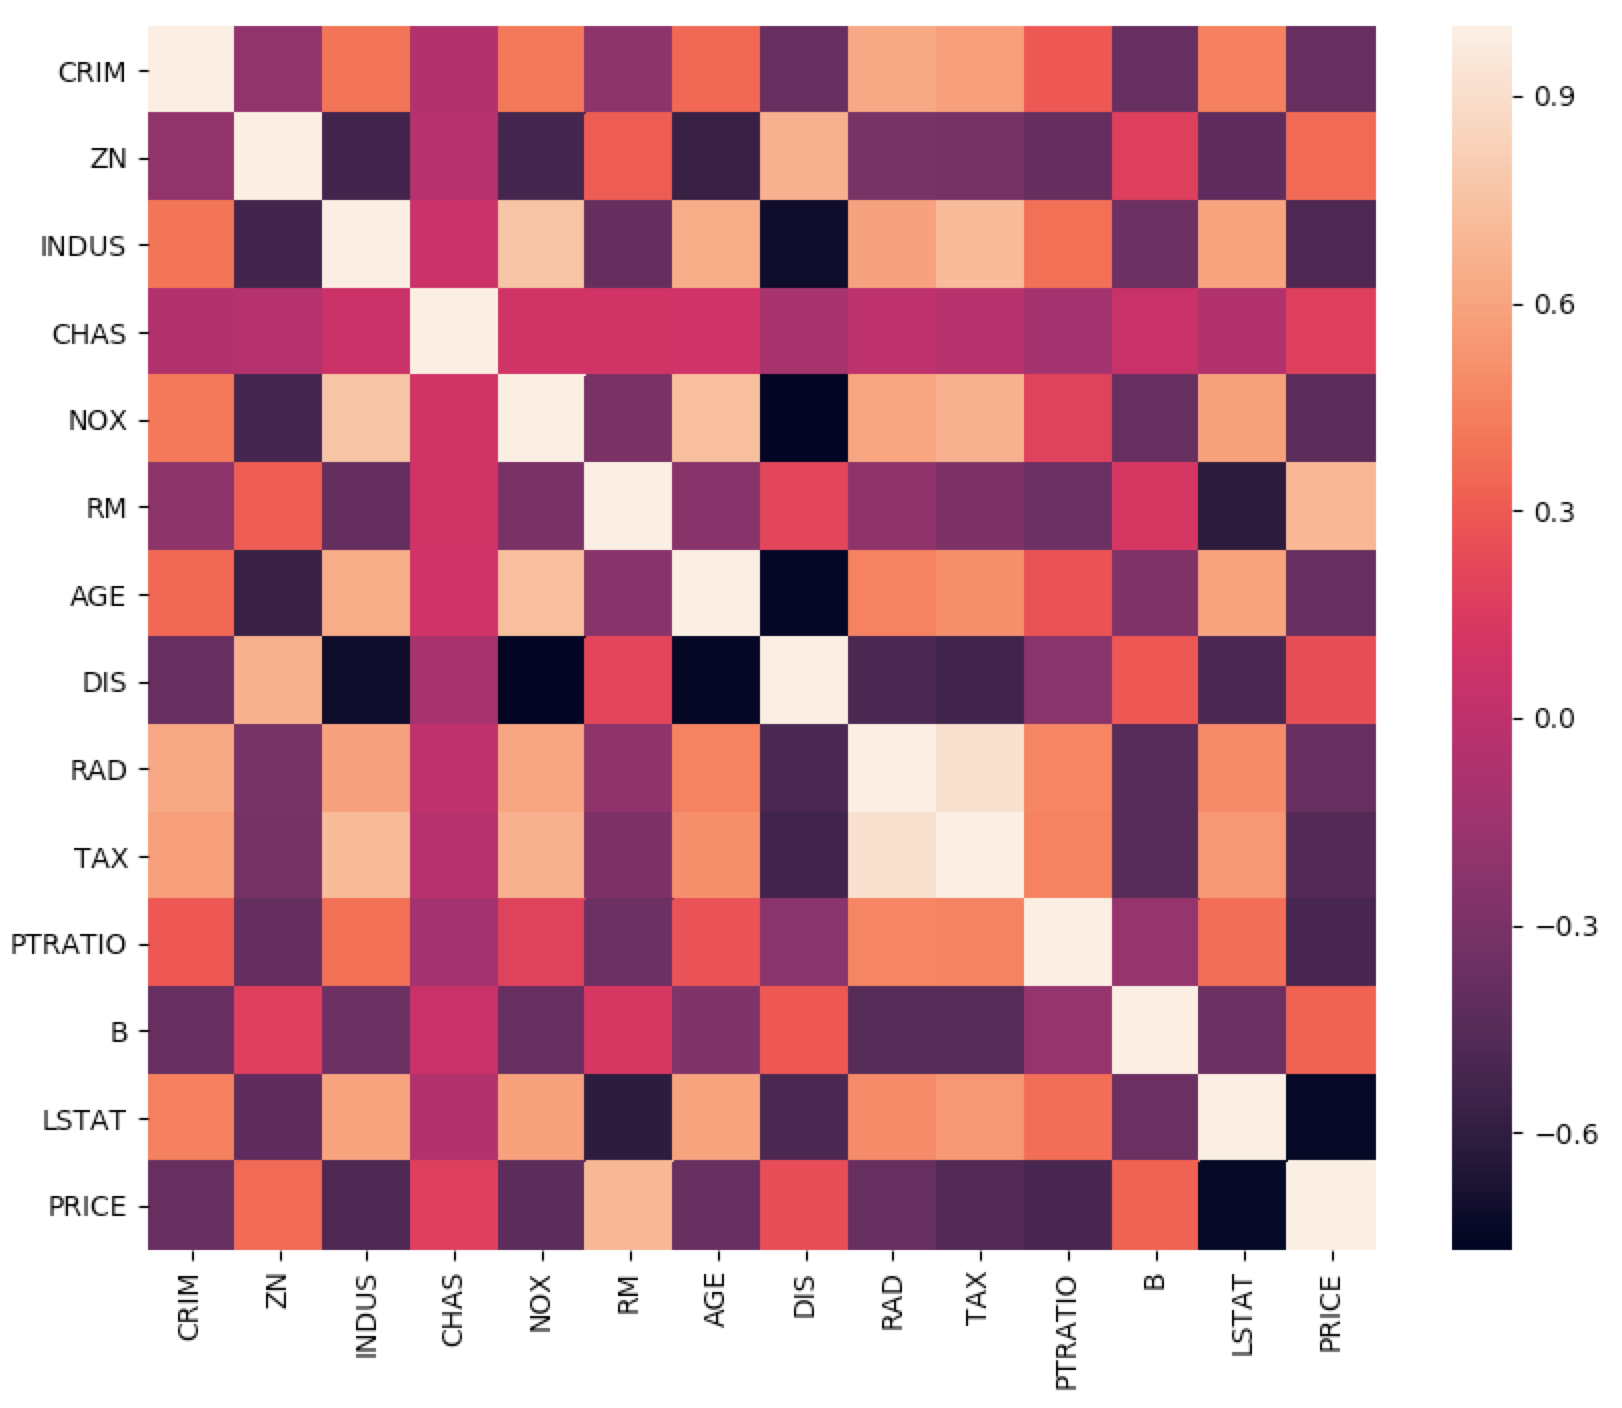
\includegraphics[width=0.65\textwidth]{boston_house_price_correlation}\\
RM: average number of rooms per dwelling
\end{center}
\end{frame}

\begin{frame}{Boston House Price dataset}
Price distribution\\
\begin{center}
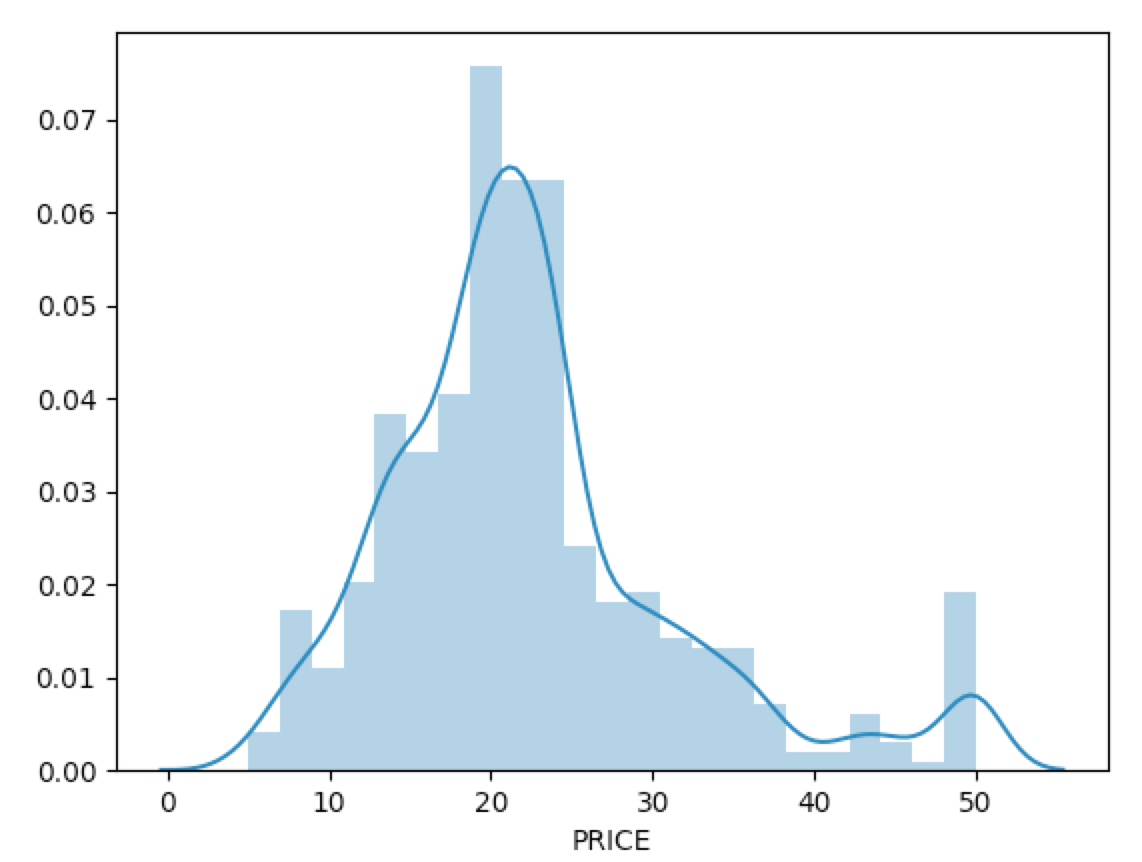
\includegraphics[width=0.80\textwidth]{boston_distr}\\
\end{center}
\end{frame}

\begin{frame}{Logistic Regression vs. Linear Regression}
Common demand in practice:
\begin{itemize}
\item there's some data existing
\item learn the concept behind it, classify new samples
\end{itemize}
\uncover<2->{
Considering the previous Boston housing dataset: estimate probability that the price > 40. (left: linear regression, right: logistic regression\\}
\uncover<3->{
\begin{center}
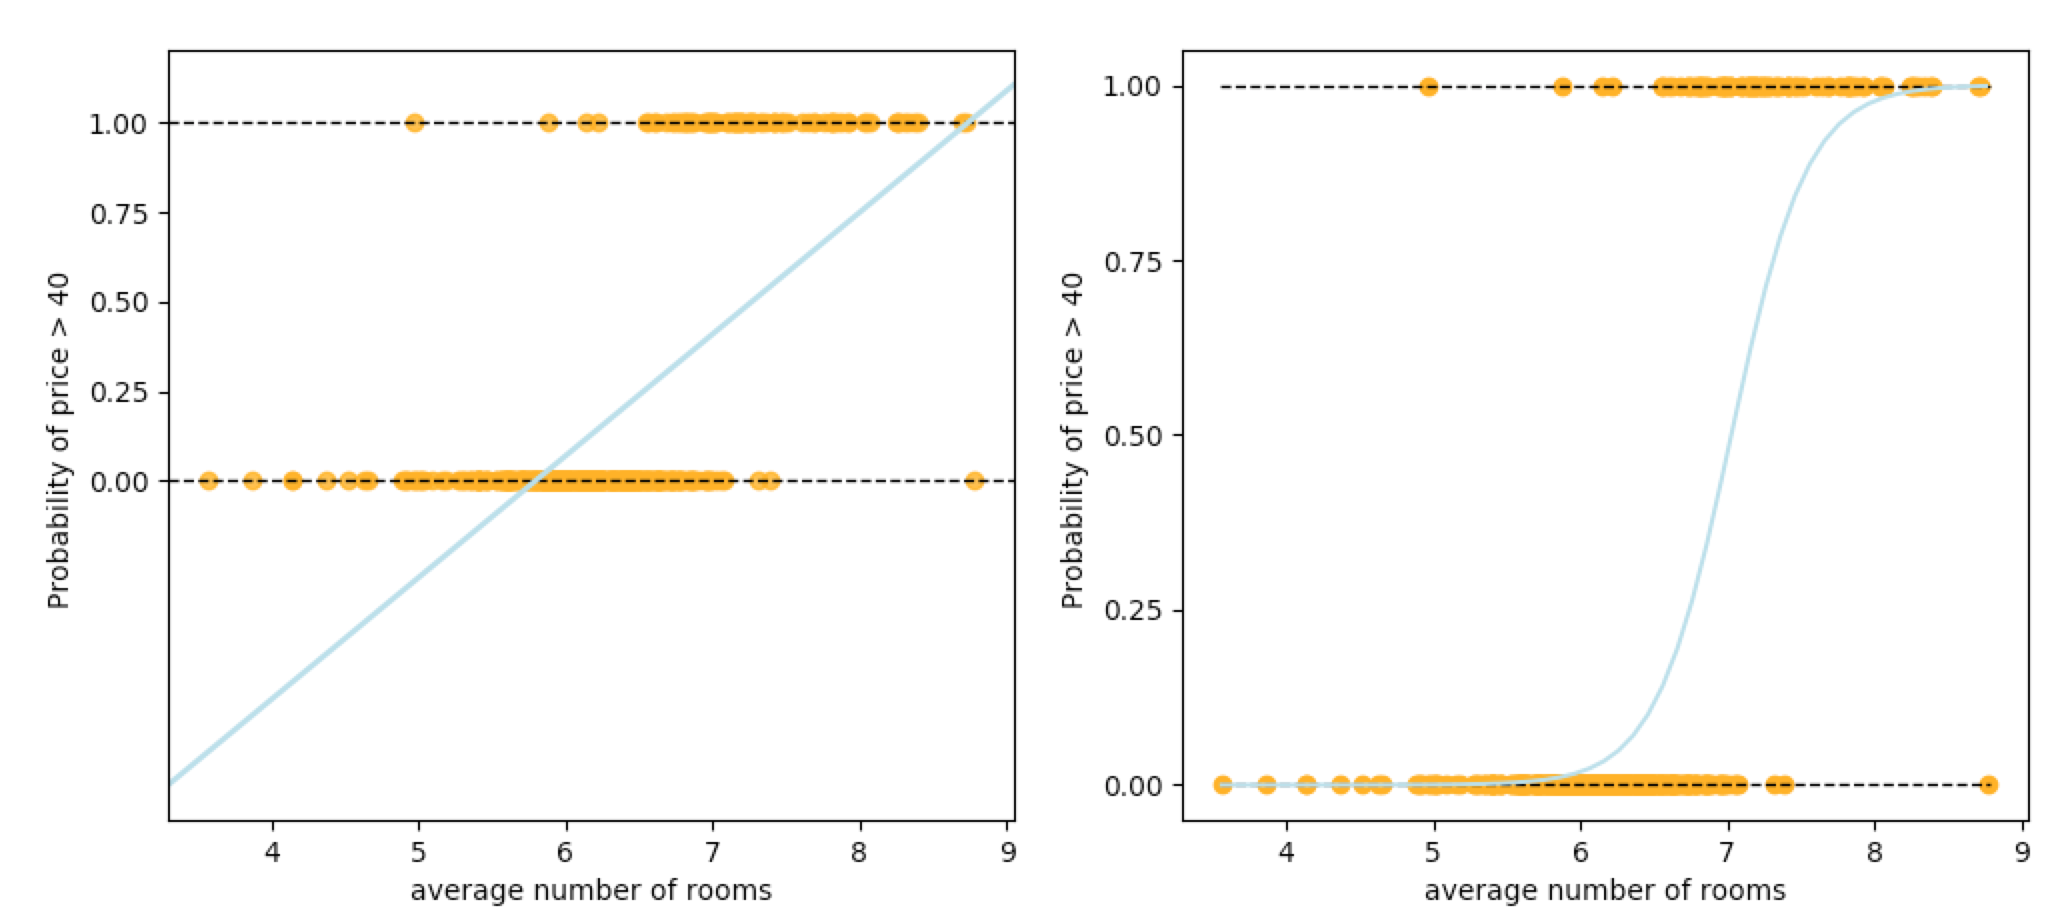
\includegraphics[width=0.9\textwidth]{log_linear_comparison}\\
\end{center}}
\end{frame}


\begin{frame}{Logistic Regression}
\begin{itemize}
\item for our linear reg. example we used $p(x) = \beta_0 + \beta_1x$
\item observation: probabilities given by linear reg. can be unreasonable $\rightarrow$ logistic regression
\item Logistic regression measures the relationship between the categorical dependent variable (p(X)) and one or more independent variables (X) by estimating probabilities using a \emph{logistic function}
\end{itemize}
\end{frame}

\begin{frame}{Logistic Regression}

\begin{block}{Logistic Function}
$\sigma(z) = \frac{e^z}{1+e^z} = \frac{1}{1+e^{-z}}$ 
\end{block}



\begin{columns}

\begin{column}{0.7\textwidth}
\begin{itemize}
\item in our example we had:\\ 
$z=\beta_0+ \beta_1x$
\item if we have $m$ explanatory variables (multiple regression) we have:\\ 
$z=\beta_0 + \sum_{i=1}^{m} \beta_i x_i$
\item for classification we can use:
$$
y=
\begin{cases}
1 & \beta_0 + \sum_{i=1}^{m} \beta_i x_i > thresh\\
0 & else
\end{cases}
$$
\emph{tresh} $\in [0,1)$ is some arbitrary threshold


\end{itemize}
\end{column}

\begin{column}{0.3\textwidth}
	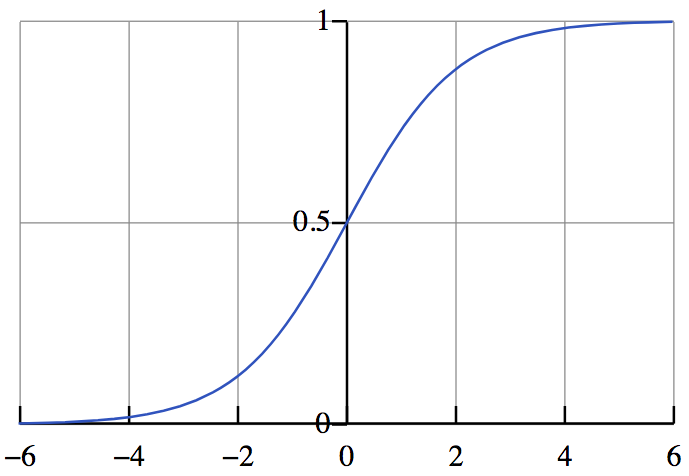
\includegraphics[width=1.1\textwidth]{logisticfunc}
\end{column}
\end{columns}
\end{frame}

\begin{frame}{Logistic Regression Side Note}
\begin{itemize}
\item how many coefficients in multiple regression are required? 
\item assess the model fit
\item do likelihood ratio-test or Wald test after fitting the coefficients
\item don't confuse multiple regression with multinomial regression
  \begin{itemize}
  \item multiple l. regression: multiple coefficients (independent variables)
  \item multinomial l. regression: dependent variable has more than two outcome categories
  \end{itemize}
\end{itemize}

\end{frame}


\begin{frame}{Observations and Example}
\begin{itemize}
\item if z is large:\\
$\sigma(z)\approx\frac{1}{1+0}=1$
\item if z is very small:\\
$\sigma(z)\approx\frac{1}{1+\infty}=0$
\uncover<1->{\item fitting logistic regression to the Boston House Price dataset yielded: $\beta_0=-27.143, \beta_1=3.862$}
\end{itemize}
\uncover<2->{\textbf{Looking for 6-room apartment:}\\
Probability of price > 40 = $\frac{1}{1+e^{-(-27.143+3.862*\textbf{6})}}=0.018$\\}
\uncover<3->{\textbf{Looking for a 8-room apartment:}\\
Probability of price > 40 = $\frac{1}{1+e^{-(-27.143+3.862*\textbf{9})}}=0.999$\\}
\uncover<4->{$\Rightarrow$ \textbf{But how do we fit our LR model?}}

\end{frame}

\begin{frame}{Fitting in Logistic Regression}
How to find the regression coefficients?
\begin{itemize}
\item unlike in linear regression we can't find a closed-form solution for logistic regression
\item instead, iterative numerical method must be used
\item we could use non-linear least squares but
\item more common to use is Maximum likelihood estimation
\item typically: Newton's method, gradient descent or L-BFGS
\end{itemize}
\end{frame}

\begin{frame}{Maximum Likelihood Estimation}
Given the data $\{(x_1, y_1), ..., (x_m, y_m)\}$ with $x_i,y_i \in \mathbb{R}^{n_x+1}$ and $x_0 = 1$ we want to find parameters $\theta=[\beta_0, \beta_1,...,\beta_{n_x}]^T$ that maximize the (conditional) likelihood of class labels $Y$ given the training data $X$.

\begin{itemize}
\uncover<1->{\item MLE attempts to find the parameter values that maximize the likelihood function (=make the data most probable), given the data:
$\hat{\theta} = \argmax_{\theta \in \Theta} \mathcal{L}(\theta; X)$
}
\uncover<2->{\item be $\hat{y}=\frac{1}{1+e^{-\theta^TX}}$}
\uncover<3->{\item in our case, the likelihood is maximized when we minimize the errors between $y$ and $\hat{y}$}
\uncover<4->{\item using the standard squared error
  \begin{center}
  $L(\hat{y},y) = \frac{1}{2}(\hat{y}-y)^2$\\
  \end{center}
we want the expression to be as small as possible}
\end{itemize}

\end{frame}

\begin{frame}{Maximum Likelihood Estimation}
Given the data $\{(x_1, y_1), ..., (x_m, y_m)\}$ with $x_i,y_i \in \mathbb{R}^{n_x+1}$ and $x_0 = 1$ we want to find parameters $\theta=[\beta_0, \beta_1,...,\beta_{n_x}]^T$ that maximize the (conditional) likelihood of class labels $Y$ given the training data $X$.

\begin{itemize}
\item for maximum likelihood we define the log-likelihood as follows (\textbf{loss function}):
  \begin{center}
  $L(\hat{y}, y) = - \big[y \log \hat{y} + (1-y) \log (1-\hat{y})\big]$
  \end{center}
\uncover<1->{\item intuition:
  \begin{itemize}
  \item minimizing a negative quantity = maximizing a positive quantity
  \item if y=1: $L(\hat{y},y)=-1 \log \hat{y} \rightarrow$ we want large $\hat{y}$
  \item if y=0: $L(\hat{y},y)=-\log(1-\hat{y}) \rightarrow$ we want small $\hat{y}$
  \end{itemize}}

\end{itemize}
\end{frame}


\begin{frame}{Maximum Likelihood Estimation(2)}
Given the data $\{(x_1, y_1), ..., (x_m, y_m)\}$ with $x_i,y_i \in \mathbb{R}^{n_x+1}$ and $x_0 = 1$ we want to find parameters $\theta=[\beta_0, \beta_1,...,\beta_{n_x}]^T$ that maximize the (conditional) likelihood of class labels $Y$ given the training data $X$.

\begin{itemize}
\item for maximum likelihood we define the log-likelihood as our \textbf{loss function}: 
  \begin{center}
  $L(\hat{y}, y) = - \big[y \log \hat{y} + (1-y) \log (1-\hat{y})\big]$
  \end{center}
\item intuition  
\uncover<2->{\item over the entirety of our data this yields the \textbf{cost function:}\\
\begin{center}
$J(\theta)=\frac{1}{m}\sum_{i=1}^{m} L(\hat{y_i},y_i)$
\end{center}
which for example can be minimized with gradient descent (later)\\
$\rightarrow$ yields the maximum likelihood estimates $\theta$ 
}
\end{itemize}
\end{frame}

\begin{frame}{Logistic Regression Optimization}
\begin{itemize}
\item the standard squared loss function is \textbf{non-convex}
\item the log-likelihood is \textbf{convex}
\item what does it mean? Some simplified examples:
% convexity: given two arbitrary points on the graph, the graph lies above or on a line that is formed by those two points 
\end{itemize}

\uncover<1->{\begin{center}
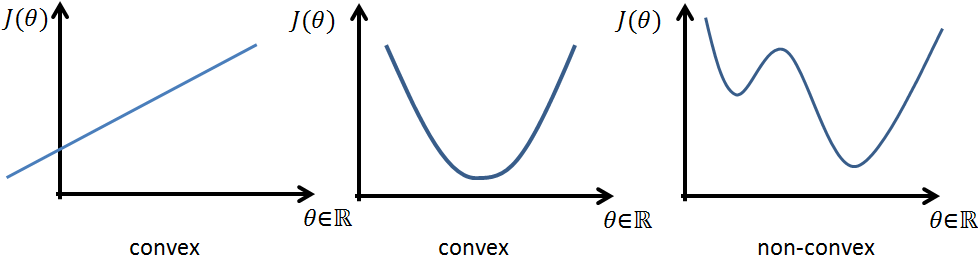
\includegraphics[width=1\textwidth]{convexity}\\
\end{center}}

\uncover<2->{
\begin{itemize}
\item log-likelihood and gradient descent (or any other iterative numerical optimization algorithm)
$\rightarrow$ yields optimal coefficients
\end{itemize}}
\end{frame}

\begin{frame}{Gradient Descent}
\begin{itemize}
\item used to find a minimum of a function
\uncover<2->{\item steps are taken in proportion to the negative of the (approx.) gradient (if positive: gradient ascent)}
\uncover<3->{\item given points $x$, an initial guess $x_0$ and a learning rate $\alpha$, gradient descent is defined as:
$$x_{n+1} = x_n - \alpha \nabla F(x_n)$$}
\uncover<4->{\item we subtract from $x$ since we want to 'move' against the gradient towards the minimum}
\uncover<5->{\item it follows for small $\alpha$: $F(x_n) \geq F(x_{n+1})$}
\end{itemize}
\end{frame}

\begin{frame}{Gradient Descent Example}
\begin{center}
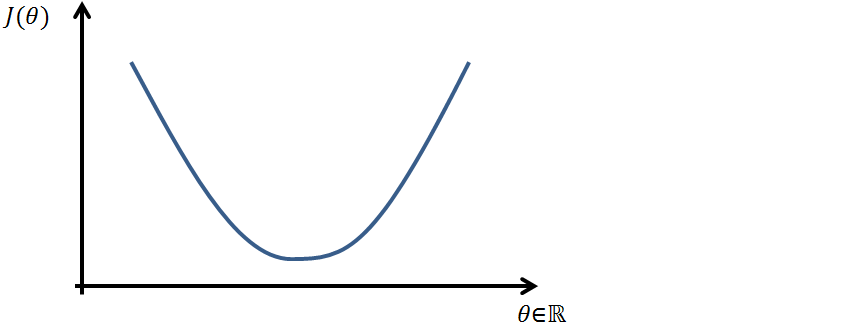
\includegraphics[width=1.1\textwidth]{gd0}
\end{center}
\end{frame}

\begin{frame}{Gradient Descent Example}
\begin{center}
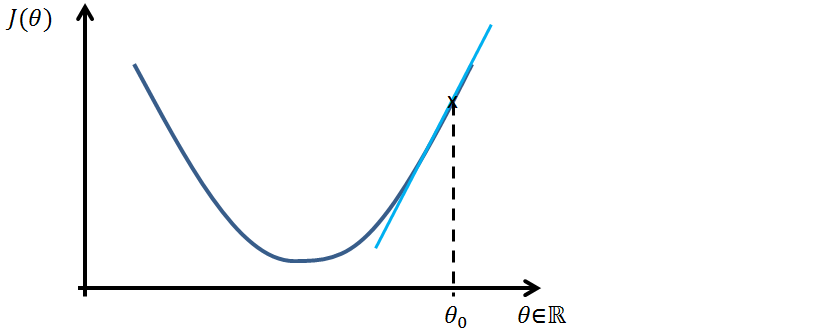
\includegraphics[width=1.1\textwidth]{gd1}
\end{center}
\end{frame}


\begin{frame}{Gradient Descent Example}
\begin{center}
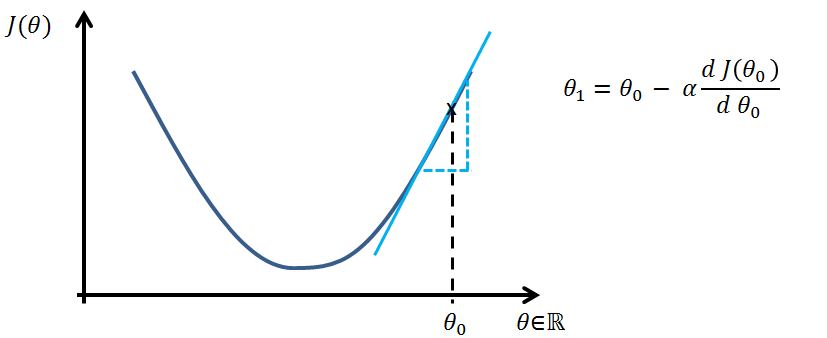
\includegraphics[width=1.1\textwidth]{gd2}
\end{center}
\end{frame}


\begin{frame}{Gradient Descent Example}
\begin{center}
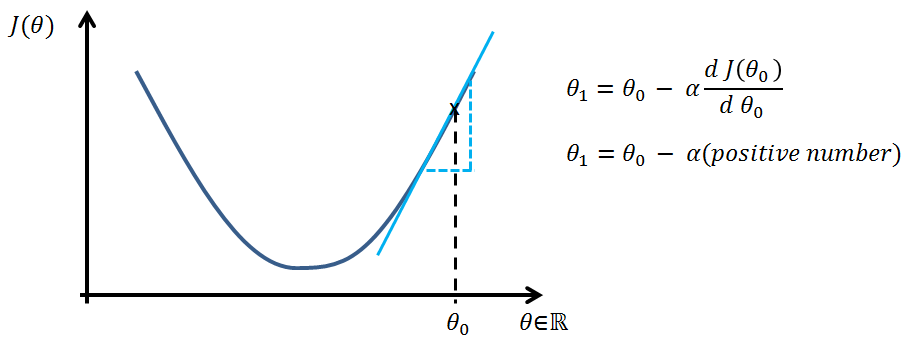
\includegraphics[width=1.1\textwidth]{gd3}
\end{center}
\end{frame}

\begin{frame}{Gradient Descent Example}
\begin{center}
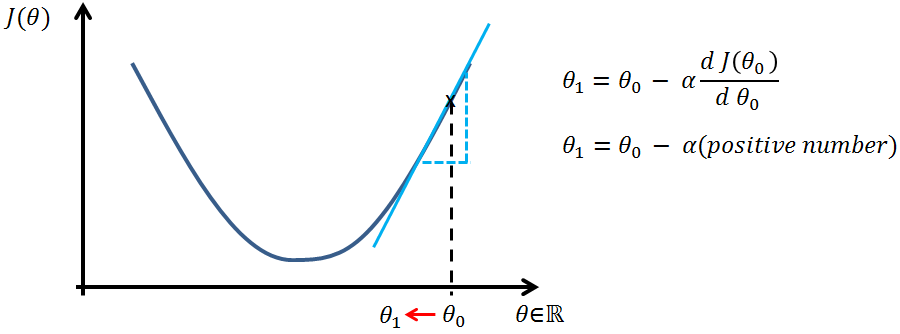
\includegraphics[width=1.1\textwidth]{gd4}
\end{center}
\end{frame}

\begin{frame}{Gradient Descent Example}
\begin{center}
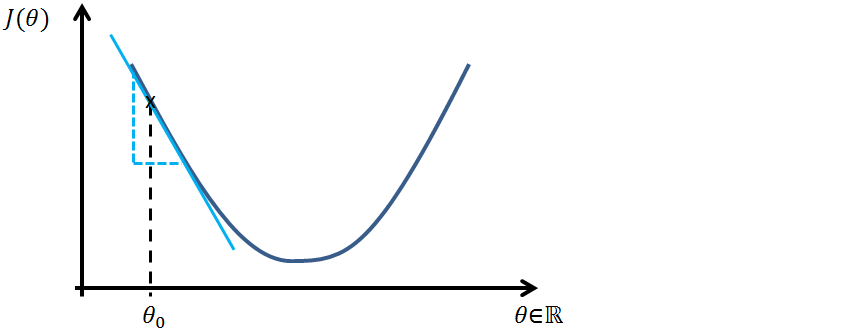
\includegraphics[width=1.1\textwidth]{gd5}
\end{center}
\end{frame}

\begin{frame}{Gradient Descent Example}
\begin{center}
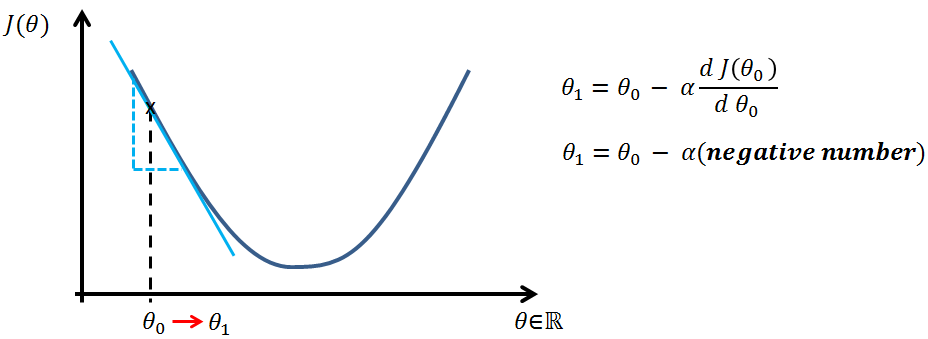
\includegraphics[width=1.1\textwidth]{gd6}
\end{center}
\end{frame}


\begin{frame}{Gradient Descent Questions}
\begin{center}
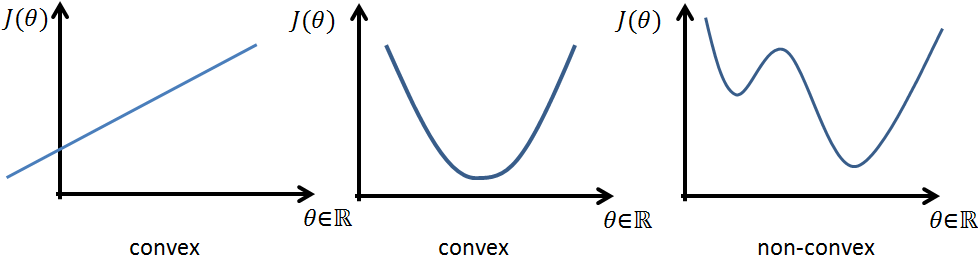
\includegraphics[width=0.8\textwidth]{convexity}
\end{center}

\begin{itemize}
\uncover<1->{\item What can be an issue when gradient descent is used with non-convex functions?}
\uncover<2->{\item What behavior can be caused by a small/large learning rate? Remember: $$x_{n+1} = x_n - \alpha \nabla F(x_n)$$}
\end{itemize}
\end{frame}

\begin{frame}{Gradient Descent Dimensionality}
Keep in mind that we usually operate on highly dimensional problems. 2d parameter space:
\begin{center}
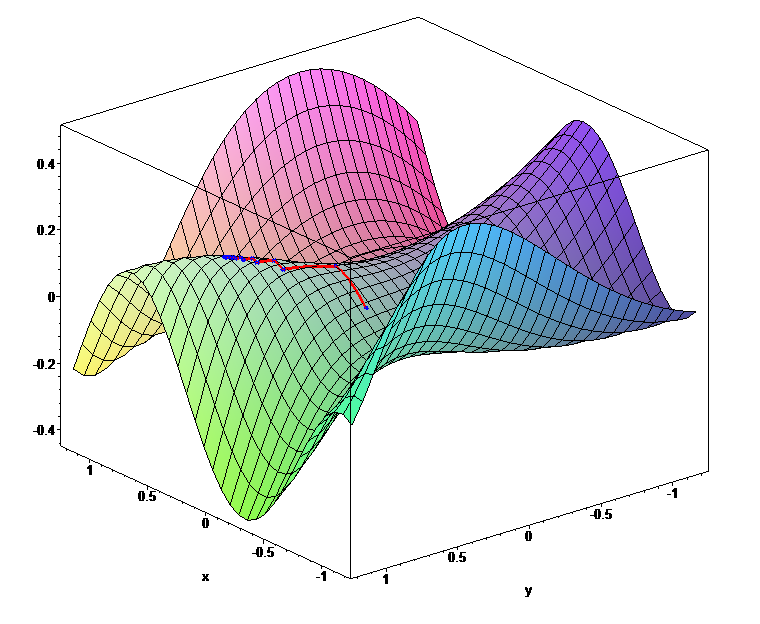
\includegraphics[width=0.5\textwidth]{gd_surface}
\end{center} \cite{WikiOverfitting}
Deep neural networks can have millions of parameters
\end{frame}

\begin{frame}{Logistic Regression in Practice}
\begin{itemize}
\item LR for handwritten digits recognition
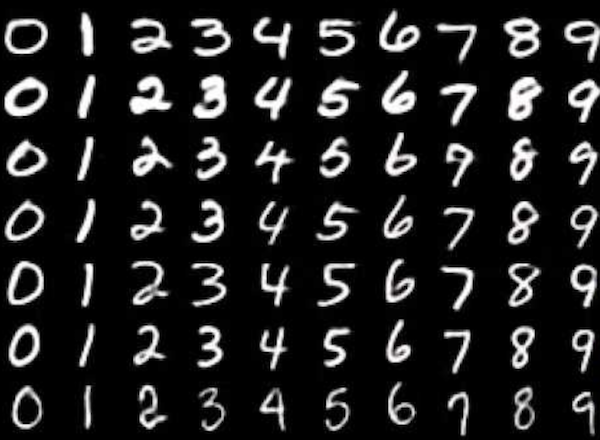
\includegraphics[width=0.3\textwidth]{lr_app1} [LeCun et al., 1998, MNIST]
\item LR for cancer detection [Stainvas et al., 2014]
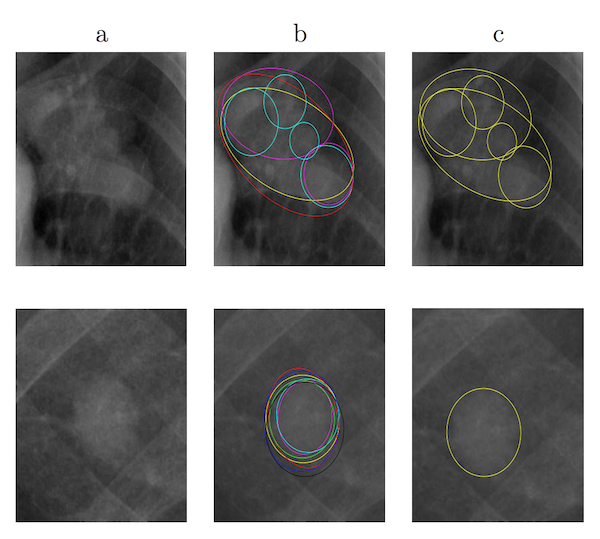
\includegraphics[width=0.4\textwidth]{lr_app2}
\end{itemize}
\end{frame}


\subsection{Neural Networks and Deep Learning}
\begin{frame}{(Artificial) Neural Networks}
\begin{itemize}
\uncover<1->{\item collection of \textbf{interconnected nodes} (artificial neurons)}
\uncover<2->{\item each connection can transmit a \textbf{signal} from one node to another}
\uncover<3->{\item the signal at a connection is a real number and the output of each neuron is calculated by a \textbf{non-linear function of the sum of its inputs}}
\uncover<4->{\item each connection also has a weight that amplifies or damps the signal}
\uncover<5->{\item NNs typically arranged into \textbf{layers}}
\uncover<6->{\item NNs can be used for \textbf{regression} and \textbf{classification} (and more)}
\uncover<7->{\item typically trained via the \textbf{backpropagation algorithm}}
\uncover<8->{\item NNs can be seen as \textbf{non-linear function approximators}}
\end{itemize}
\end{frame}

\begin{frame}{(Artificial) Neural Networks Example}
Single-layer neural network: input and output layer\\
Multi-layer neural network\footnote{sometimes called multi-layer perceptron}  (below): input, hidden, output layer
\begin{center}
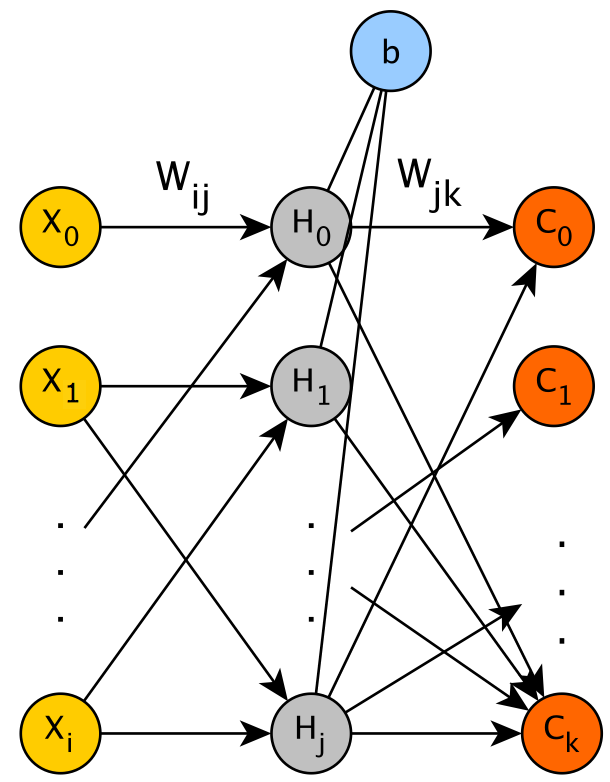
\includegraphics[width=0.3\textwidth]{basic_ff_nn}
\end{center}
\begin{itemize}
\item nodes of two adjacent layers are \emph{fully-connected}
\item can be seen as feature extractor (weights allow/restrict certain inputs)
\end{itemize}
\end{frame}

\begin{frame}{Neural Network Model Classes}
\begin{itemize}
\item artificial neural networks (ANN or just NN) form a large class of models, to name just a few:
\uncover<2->{
\begin{itemize}
\item feed-forward NN
    \begin{itemize}
	\item Perceptron / "Vanilla"
    \item Convolutional
    \item Autoencoder
    \end{itemize}
}
\uncover<3->{
\item recurrent NN
  \begin{itemize}
  \item Long short-term memory
  \item Bi-directional
  \end{itemize}
}
\uncover<4->{
\item undirected NN
  \begin{itemize}
  \item Deep Belief
  \item Restricted Boltzmann
  \end{itemize}
}
\uncover<5->{
\item "third generation": Spiking NN
  \end{itemize}
\item in this lecture we will focus on feed-forward NN for classification
}
\end{itemize}  
\end{frame}


\begin{frame}{Perceptron (Rosenblatt, 1957)}
\begin{itemize}
\item one of the first ANNs
\item algorithm for learning a linear binary classifier
\item positive (P) and negative (N) sets of data samples
\item input $x$ is mapped to an output value (0 or 1) which is calculated by the dot product of the weight vector $w$ and $x$
\item the output value is used to classify $x$ as either a positive or a negative instance
\end{itemize}
\end{frame}

\begin{frame}{Perceptron (Rosenblatt, 1957)}
\centering
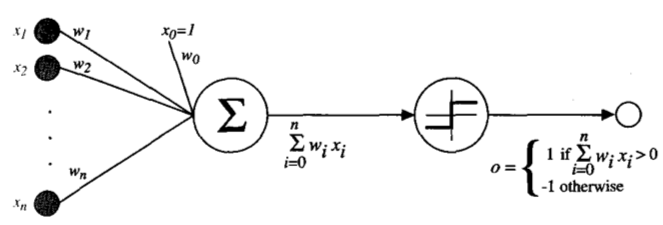
\includegraphics[width=1\textwidth]{perceptron1}\\from \cite{mitchell1997a}\\
adjustment of weights is equivalent to searching for the best decision boundary
\end{frame}

\begin{frame}{Perceptron (Rosenblatt, 1957)}
algorithm:
\begin{itemize}
\item Phase start: 
  \begin{itemize}
  \item initialize $w_0$ randomly, $t:=0$
  \item given data samples $P\cup N$ 
  \end{itemize}
\item Phase test:
  \begin{itemize}
  	\item choose $x \ in P\cup N$ randomly
	\item if $x\in P$ and $w_t \cdot x > 0 $ go to test
    \item if $x\in P$ and $w_t \cdot x \leq 0 $ go to add
    \item if $x\in N$ and $w_t \cdot x < 0 $ go to test
    \item if $x\in N$ and $w_t \cdot x \geq 0 $ go to subtract
  \end{itemize}
\item Phase add:
  \begin{itemize}
  \item set $w_{t+1} = w_t + x, t:= t+1$
  \end{itemize}
\item Phase subtract:
  \begin{itemize}
  \item set $w_{t+1} = w_t - x, t:= t+1$
  \end{itemize}
\end{itemize}
\end{frame}


\begin{frame}{Perceptron Example: Geometric Interpretation in $\mathbb{R}^2$}
\begin{itemize}
\item in the following example, all shown samples $x_i$ from $P$
\item note the dot product: $w_t \cdot x_j$, i.e. $w^0_t x^0_j + ... + w^i_t x^i_j$
(for j-th sample at time-step t and $0 < i < n$ for n-dimensional vectors)
\item sometimes extension used: construct a supporting set $N' = \{x' | x' = -x, \forall x \in N\}$\\
\item now all samples are correctly classified iff $x \cdot w > 0, \forall x \in N' \cup P$
\end{itemize}
\end{frame}

\begin{frame}{Perceptron Example: Geometric Interpretation in $\mathbb{R}^2$}
\centering
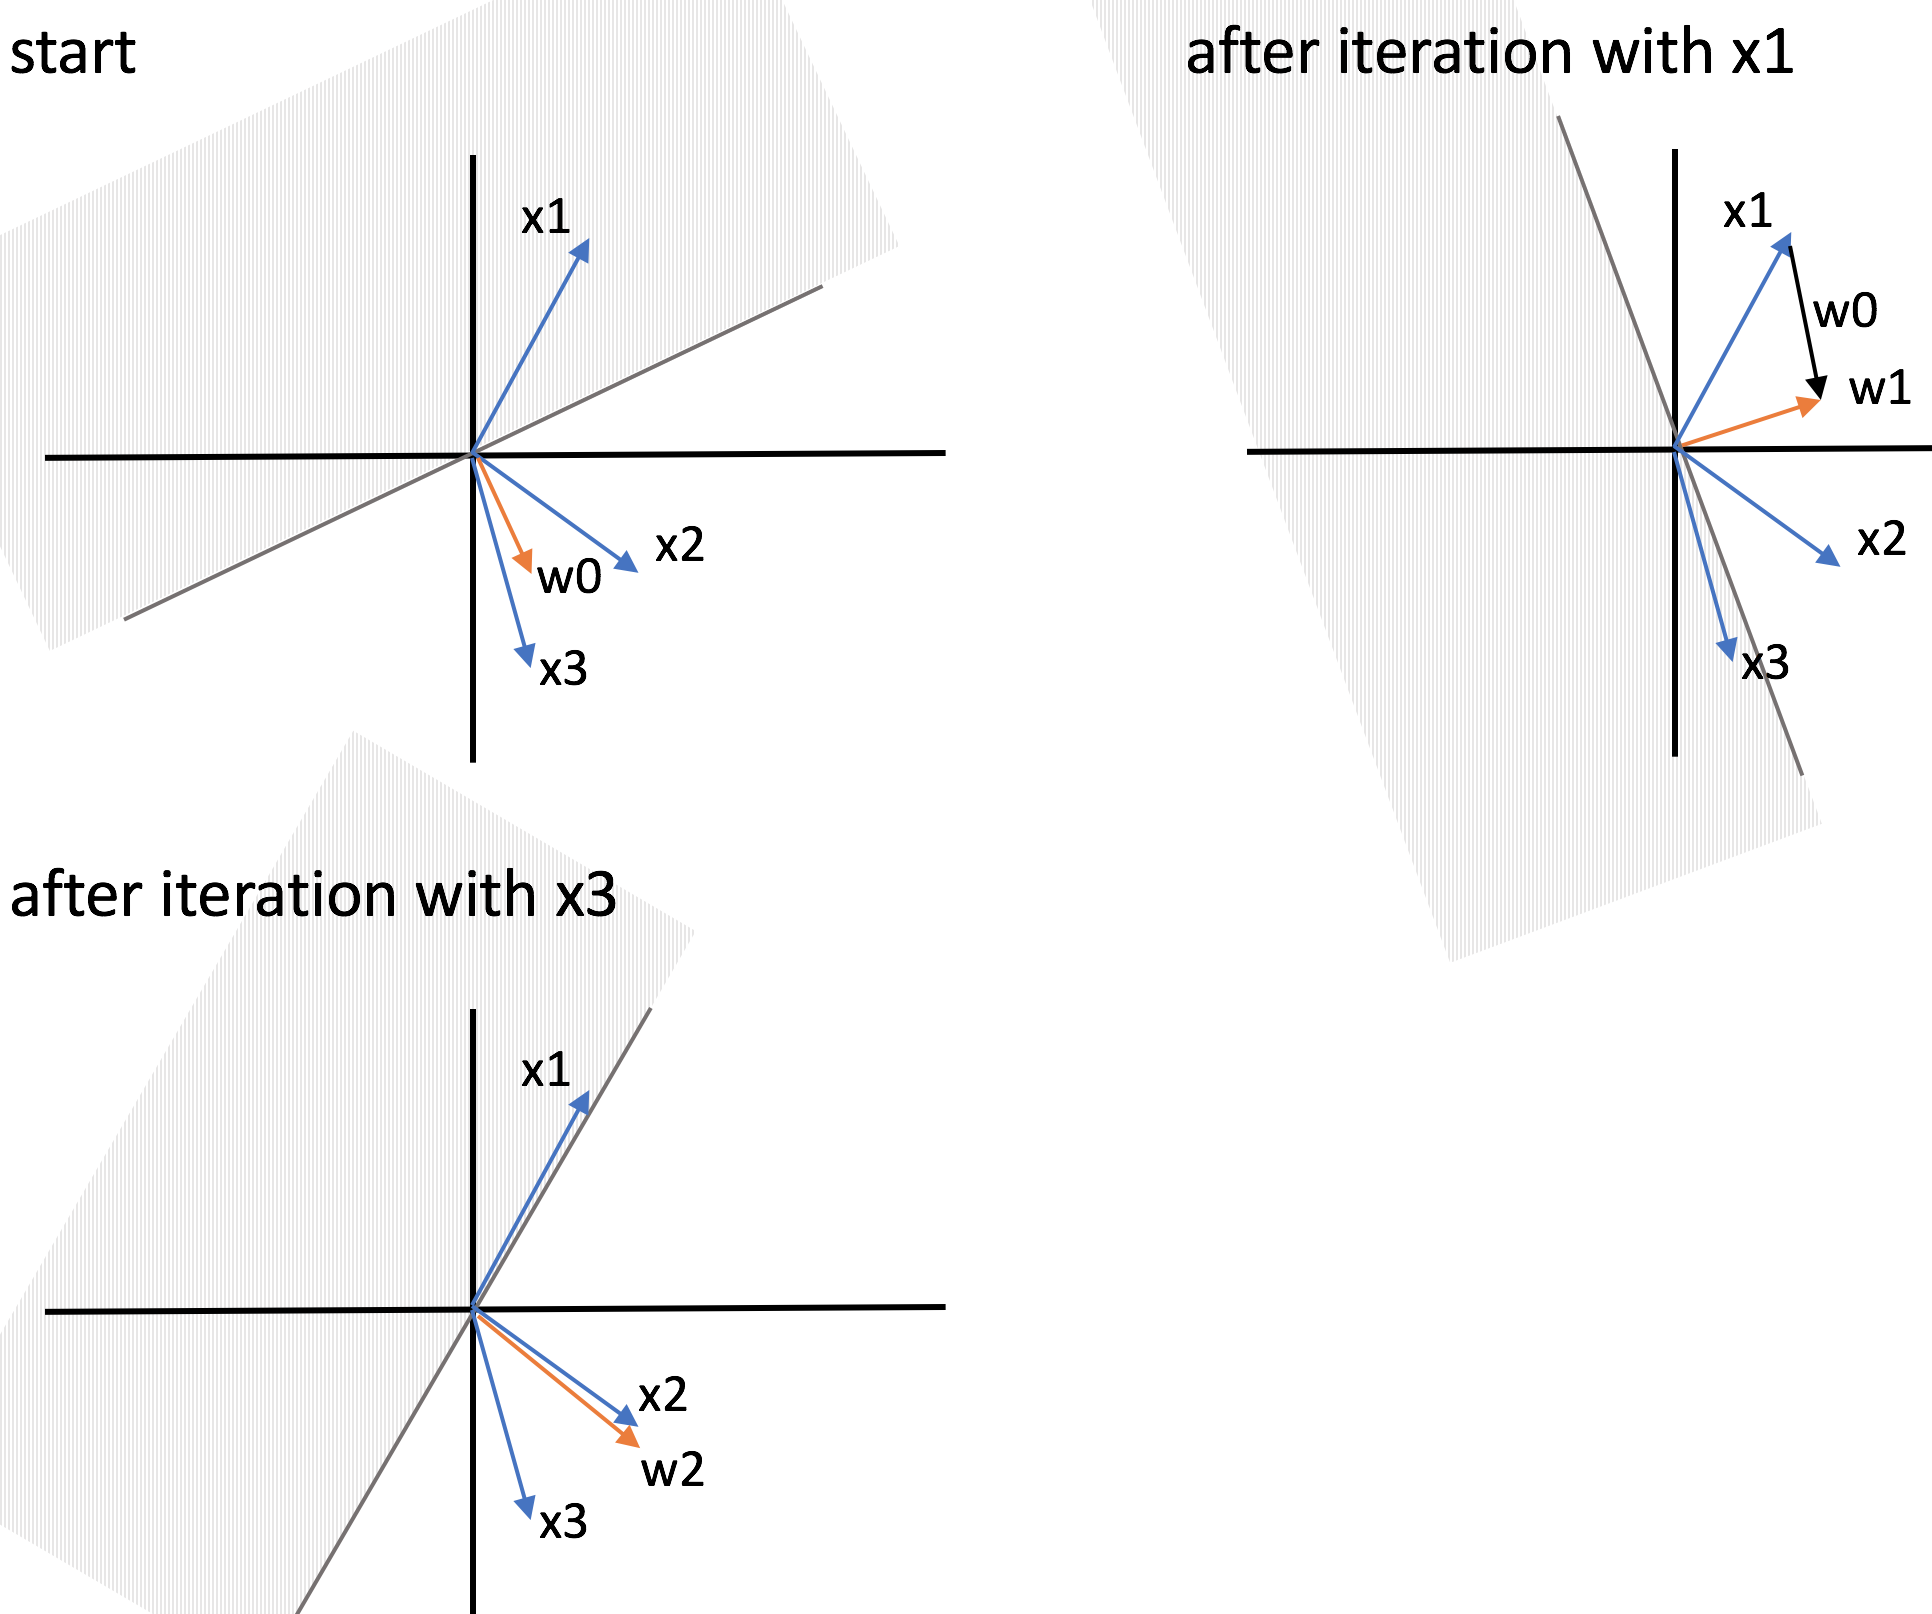
\includegraphics[width=0.8\textwidth]{perceptron2}
\end{frame}




\begin{frame}{Perceptron Review}
\begin{itemize}
\uncover<1->{\item slow adjustment if $|w| >> |x| \Rightarrow$ solution: normalize vectors}
\uncover<2->{\item collinear $x$ vectors will result in oscillation $\Rightarrow$ slow convergence}
\uncover<3->{\item if samples are not linearly separable there's no convergence $\Rightarrow$ use delta-rule to overcome this issue}
\uncover<4->{\item the delta-rule is an update-rule that uses gradient descent to search the hypothesis space and to find the weights that best fit the samples (not discussed here)}
\uncover<2->{\begin{center}
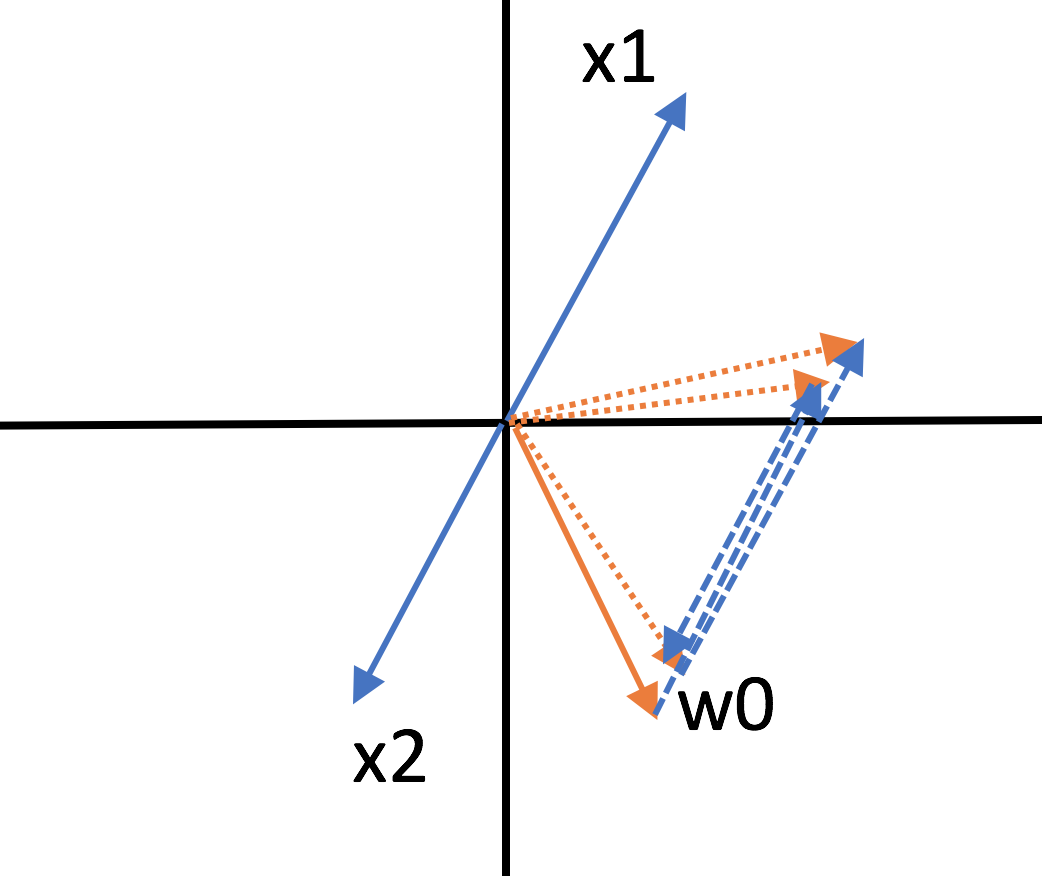
\includegraphics[width=0.4\textwidth]{perceptron3}
\end{center}}
\end{itemize}
\end{frame}


\begin{frame}{Relation between Logistic Regression and NN}
\uncover<1->{\textbf{artificial neuron:} (arbitrary activation function)\\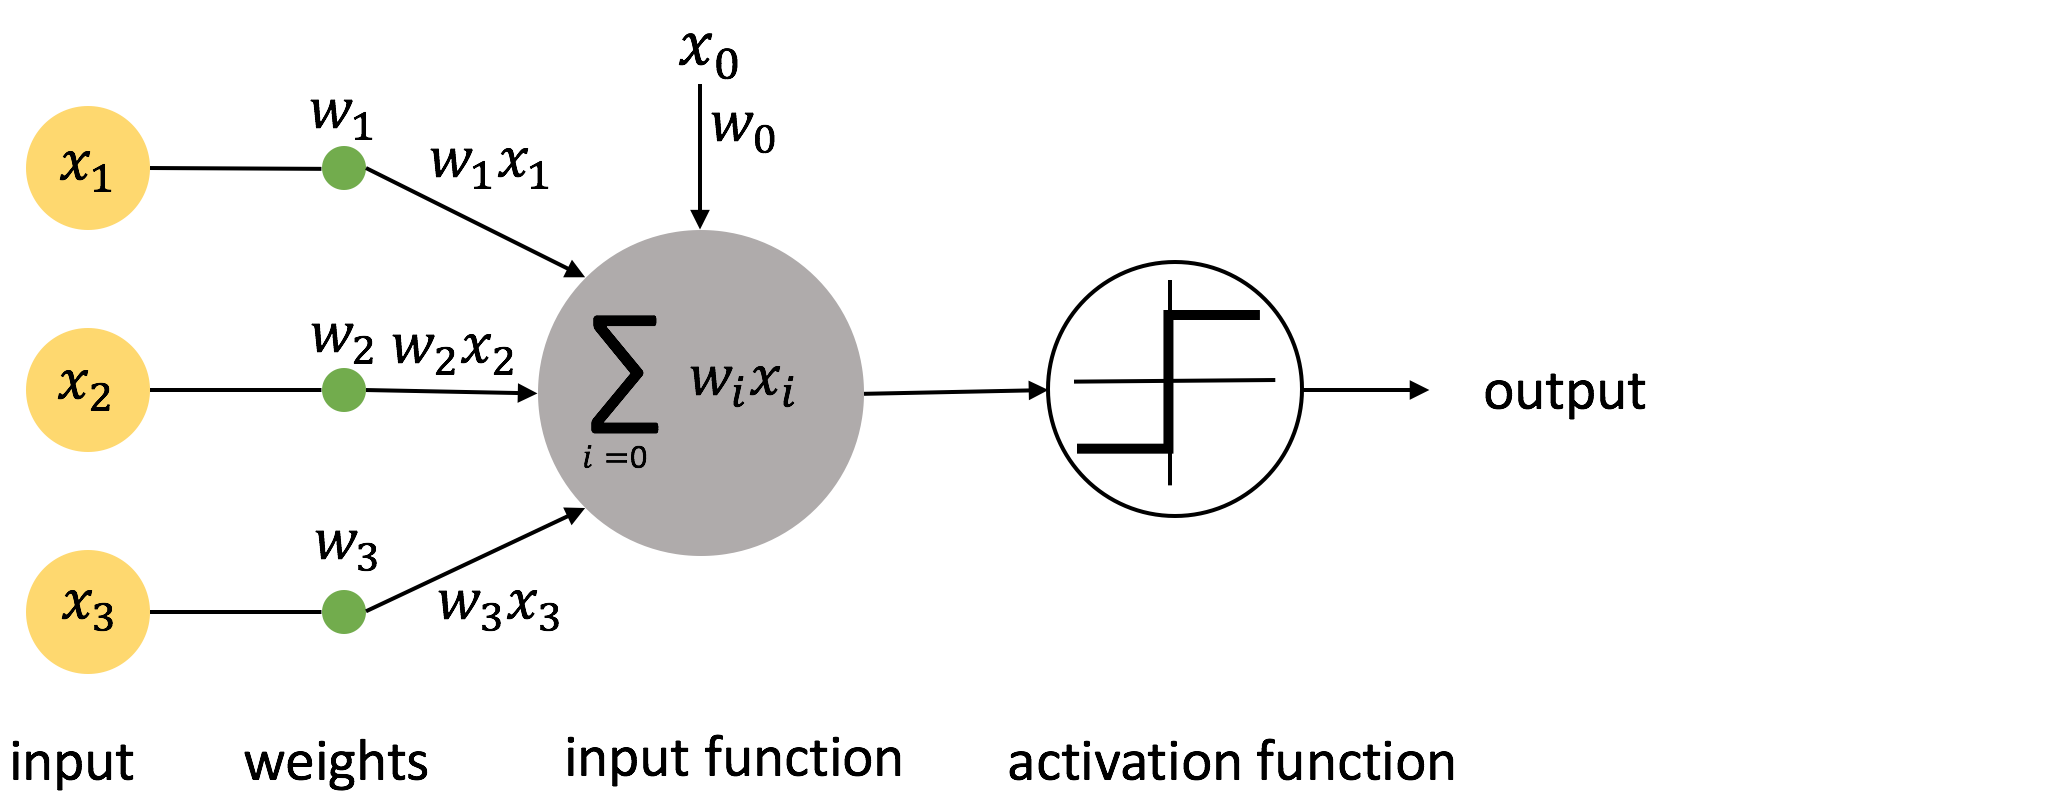
\includegraphics[width=0.62\textwidth]{artificial_neuron}}\\
\uncover<2->{\textbf{logistic regression:} (logistic function as activation)
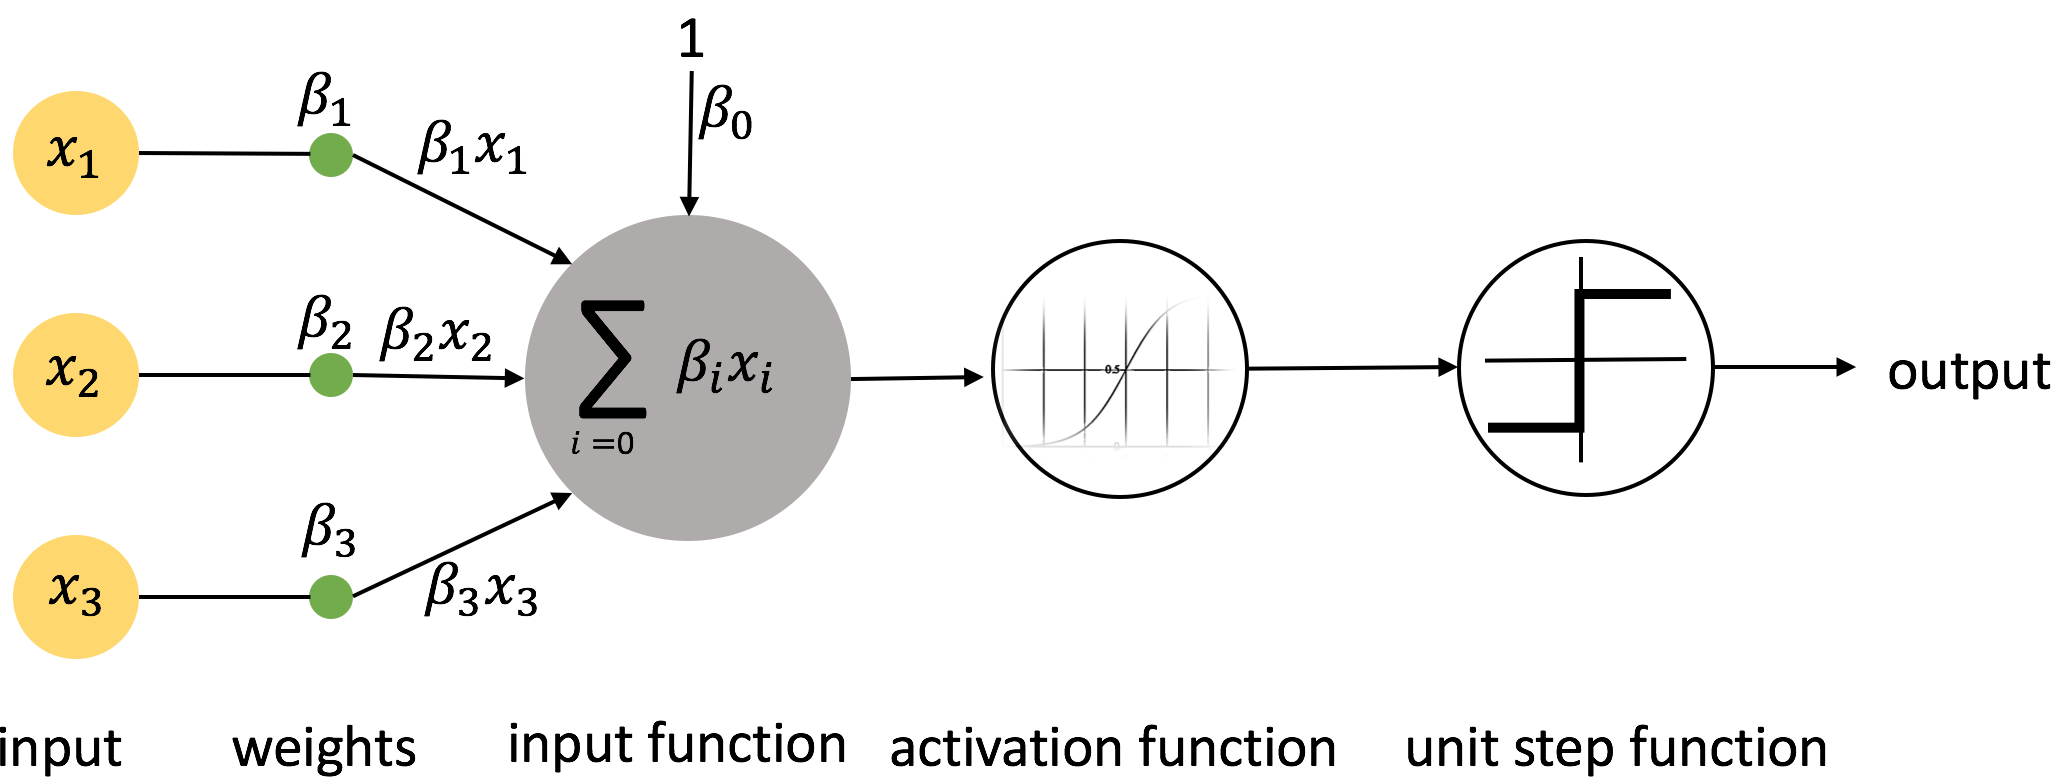
\includegraphics[width=0.75\textwidth]{logistic_regression_unit}}
\end{frame}

\begin{frame}{Activation Functions}
\uncover<1->{\begin{itemize}
\item every hidden neuron usually has an activation function
\item usually maps the resulting values to values between 0 and 1 or -1 and 1
\item can be linear or non-linear
\end{itemize}}

\uncover<2->{Why activation functions?}
\begin{itemize}
\uncover<3->{\item functions we want to model are typically non-linear}
\uncover<4->{\item increase the capacity of NNs and thus, the complexity of their functions}
\uncover<5->{\item a multi-layer NN with just linear AFs behaves like a single-layer NN with linear AFs\footnote<5->{the composition of two linear functions is itself a linear function} $\Rightarrow$ make actual use of network depth}
\end{itemize}
\end{frame}


\begin{frame}{Activation Functions}
Some activation functions:
\begin{center}
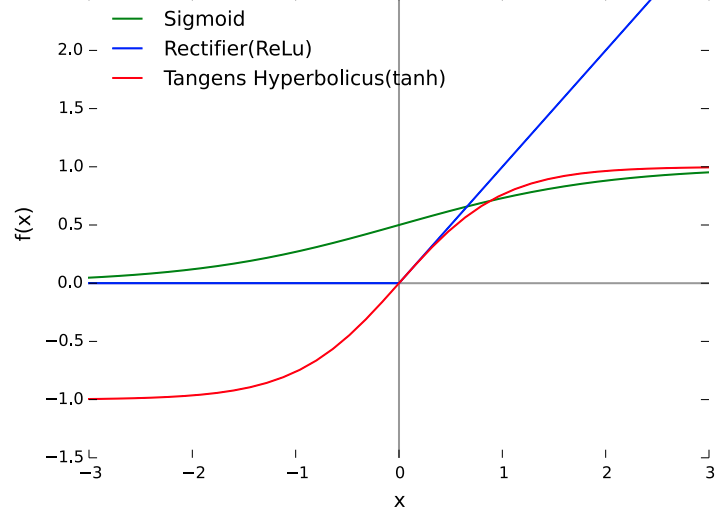
\includegraphics[width=0.7\textwidth]{activation_functions}
\end{center}
important: since we use backpropagation to train NNs, we require AFs to be differentiable
\end{frame}

\begin{frame}{Output Neurons and Classification}

\begin{center}
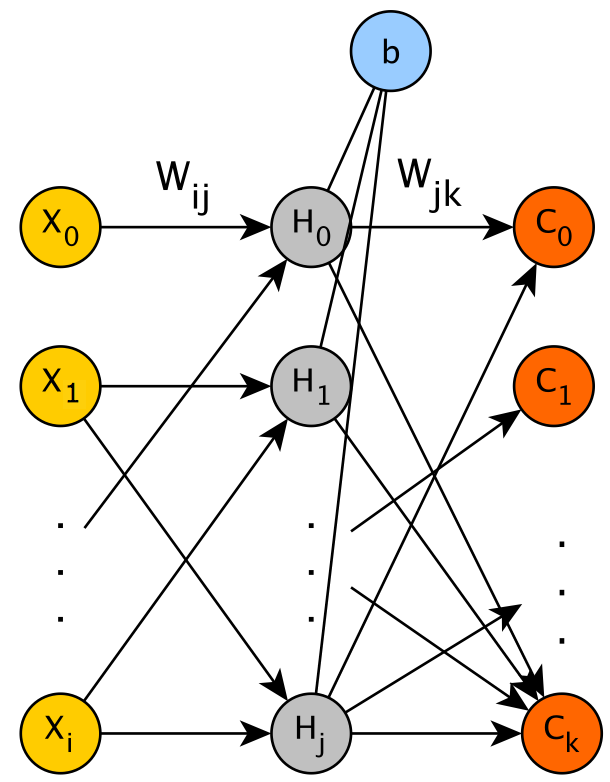
\includegraphics[width=0.3\textwidth]{basic_ff_nn}
\end{center}

\begin{itemize}
\item $k$ output neurons allow classification for $k$ different classes
\item \textbf{healthy intuition:} layers prior to the output layer map the data to a higher dimensional representation that (ideally) is linearly separable by the output neurons\footnote{which form a (k-1)-dimensional hyperplane in the k-dimensional space}
\end{itemize}
\end{frame}

\begin{frame}{Multi-layer Neural Networks and Deep Learning}
\begin{itemize}
\uncover<1->{\item a NN with at least three (input, hidden, output) is considered to be a multi-layer NN}
\uncover<2->{\item \textbf{what's the difference between neural networks and deep neural networks?}}
\uncover<3->{
  \begin{itemize}
  \item no definite answer to what "deep" is
  \item usually more than two or three hidden layers are called deep
  \item NN with no or one hidden layer is called "shallow"
  \item note: the term "deep" is time-dependent as NN tend to get deeper over time
  \end{itemize}}
\uncover<4->{\item \textbf{why go deep (and not wide)?}}
\uncover<5->{
  \begin{itemize}
  \item despite the universal approximation theorem (one "large" hidden layer suffices), deep NN work better in practice across many domains
  \item the following slides focus on deep NN but can be applied to shallow NN, too
  \end{itemize}}
\end{itemize}

\end{frame}

\begin{frame}{Cost function}
\begin{itemize}
\item remember: a \textbf{loss function} quantifies the deviation between a classification result and a target value w.r.t. a single sample
\uncover<2->{\item a \textbf{cost function} quantifies the loss w.r.t the entire dataset}
\uncover<3->{\item a set of parameters (weights) are considered optimized if the costs are 0 or can not be further reduced (convergence criteria)}
\uncover<4->{\item the loss function forms an "error surface" in which our optimization operates}
\uncover<5->{\item optimization is done via the \textbf{backpropagation algorithm}}
\uncover<6->{\item typical cost functions are:
\begin{itemize}
\item Mean Squared Error (MSE)
\item SVM (cost function)
\item \textbf{Softmax}
\end{itemize}}
\end{itemize}
\end{frame}

\begin{frame}{Softmax Cost Function}
\begin{itemize}
\item the Softmax cost function is a generalization of the binary logistic regression to multiple classes\footnote{non-linear variant of the multinomial logistic regression}
% y label can take on more than two possible values
% http://ufldl.stanford.edu/wiki/index.php/Softmax_Regression
\item Softmax yields normalized class probabilities $\Rightarrow$ probabilistic interpretation
\item let's first take a look at the \textbf{softmax function}: 

\begin{equation}
    \sigma(x_i) = \frac{e^{x_i}}{\sum_{k}^K e^{x_k}}
\end{equation}\\
$\Rightarrow$ it squashes a $K$-dimensional vector $x$ of arbitrary real values to a $K$-dimensional vector $\sigma(x)$ of real values in the range (0,1) that add up to 1
\end{itemize}
%(maybe include MNIST 10 class example)
\end{frame}

\begin{frame}{Softmax Cost Function}
Softmax function example:
\begin{center}
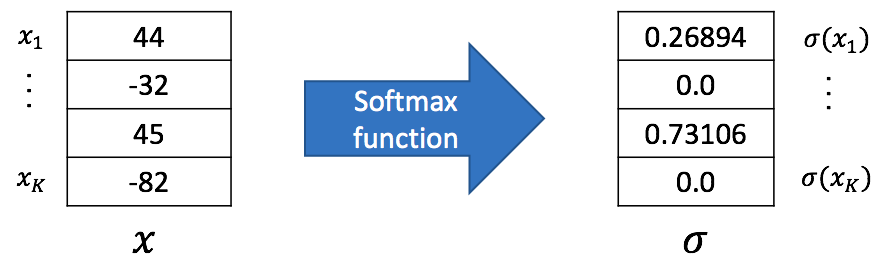
\includegraphics[width=1\textwidth]{softmax_function_example}
\end{center}
\end{frame}

\begin{frame}{Softmax Cost Function}
\begin{itemize}
\uncover<1->{\item now let $f(x_i; W) = Wx_i$ be the score function with
\begin{itemize}
\item $W$ the weights (and biases) from the NN
\item and the input vector $x_i$
\end{itemize}}
\uncover<2->{\item we use the softmax function to build the loss function
\begin{equation}
	L_i = -\log (\frac{e^{f_{y_i}}}{\sum_j^K e^{f_j}})
\end{equation}\\
where $y_i$ chooses the index of the correct label at step $i$ and $f_j$ is the $j$-th element of the class scores vector $f$}
\uncover<3->{\item intuitively, $L_i$ yields the normalized probability of class $y$ for a given input $x_i$ and parameters $W$}
\uncover<4->{\item the cost for the data is the mean of $L_i$ over all training samples}
\end{itemize}
\end{frame}

\begin{frame}{Softmax Cost Function}
\begin{itemize}
\uncover<1->{\item to complete our intuition we consider the cross entropy:}
\uncover<2->{\begin{equation}
	H(p,q) = - \sum_k p(x) \log q(x)
\end{equation}}
\uncover<3->{\item set $L_i = \log q(x)$
\item $p=[0,...,1,...0]^T$ with a single 1 at $y_i$-th position}
\uncover<4->{\item $\Rightarrow$ the softmax classifier minimizes the cross-entropy between the log probability of the predicted class $y_i$ and the true distribution $p$}
\uncover<4->{\item $\Rightarrow$ during training, the predicted distribution will be enforced to have all of its mass on the correct class}
\uncover<5->{\item minimizing the negative log prob is equal to maximizing the log prob (of choosing the correct class)}
\end{itemize}
\end{frame}

\begin{frame}{Softmax Cost Function Example}
\begin{center}
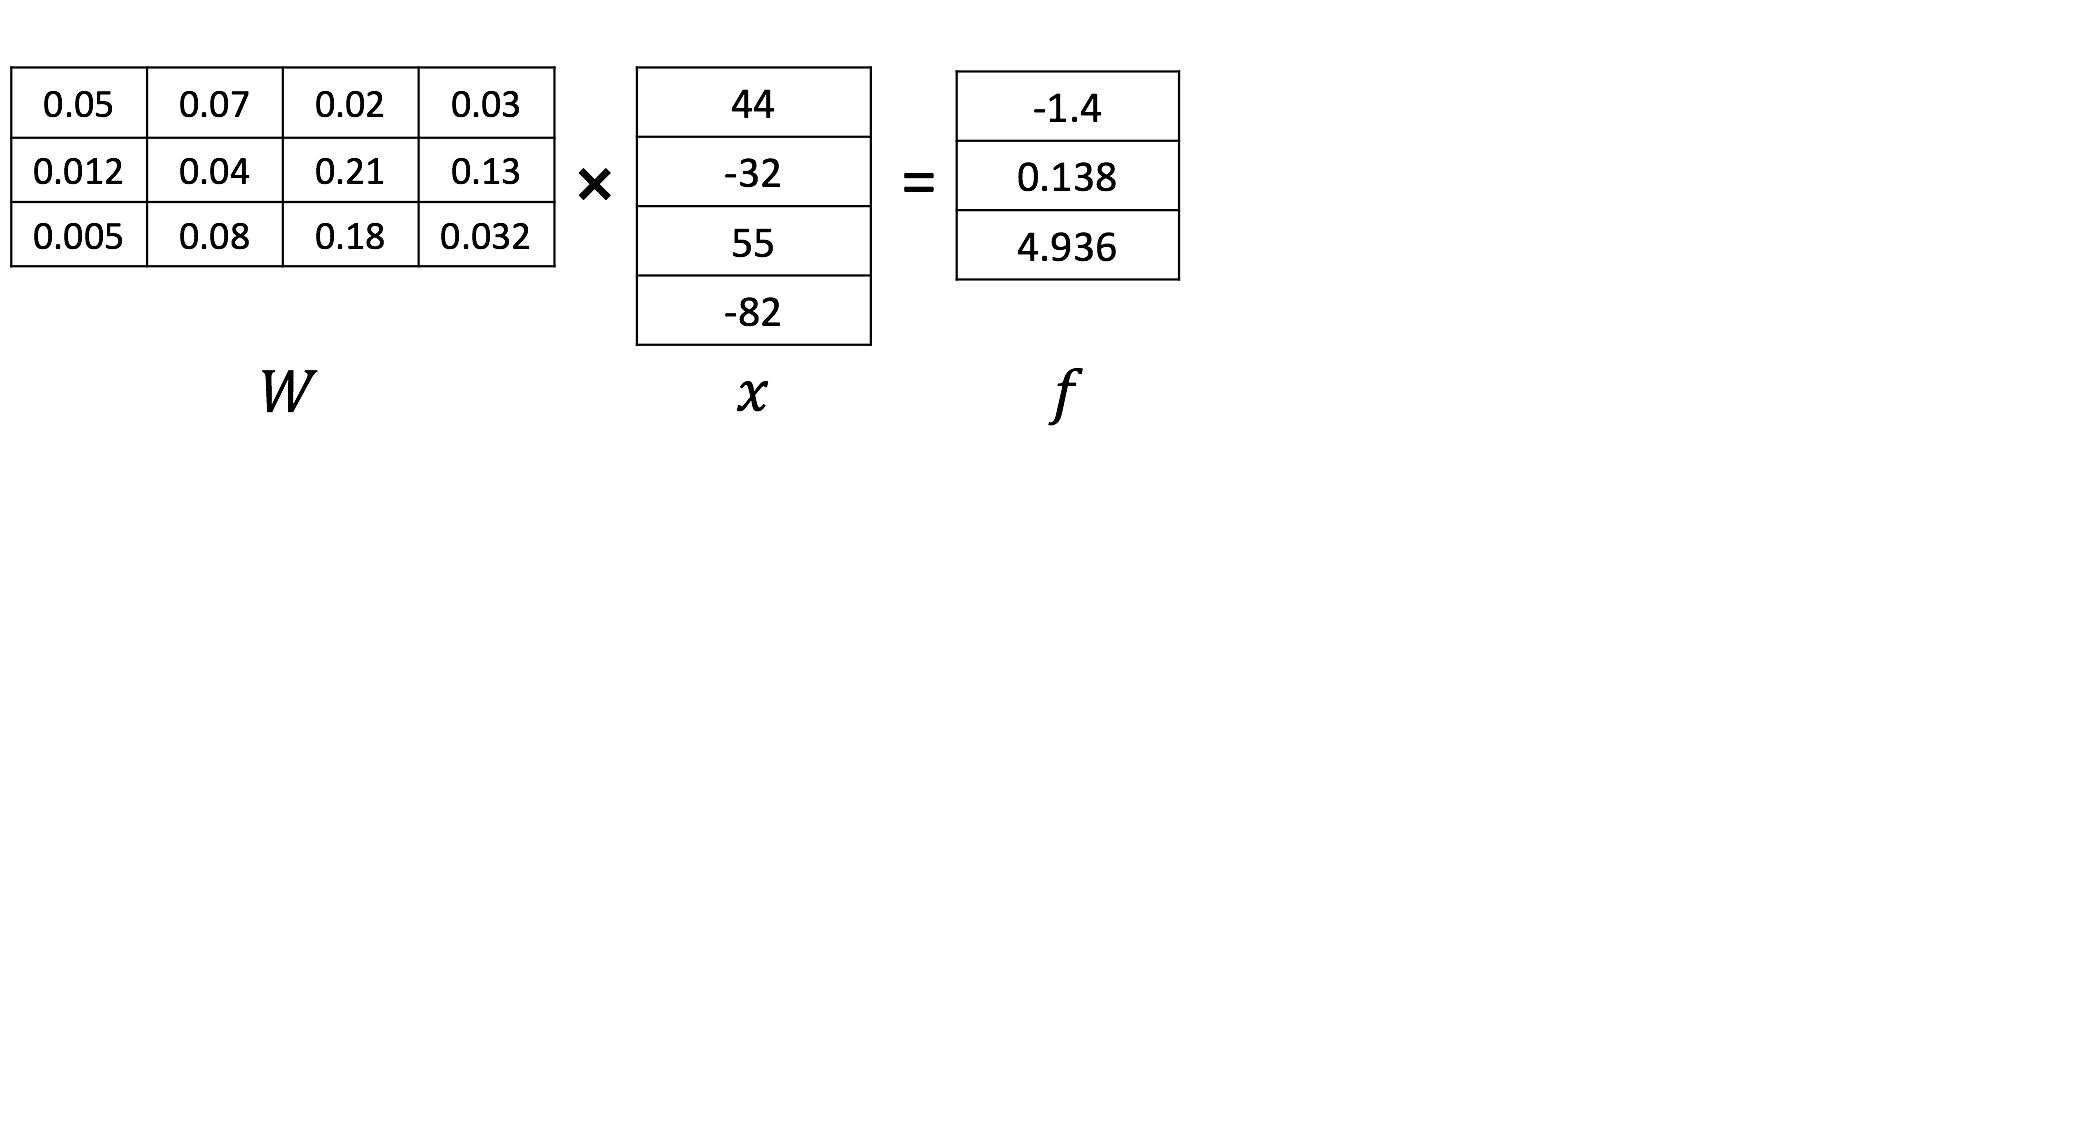
\includegraphics[width=1.05\textwidth]{softmax_example1}
\end{center}
\end{frame}

\begin{frame}{Softmax Cost Function Example}
\begin{center}
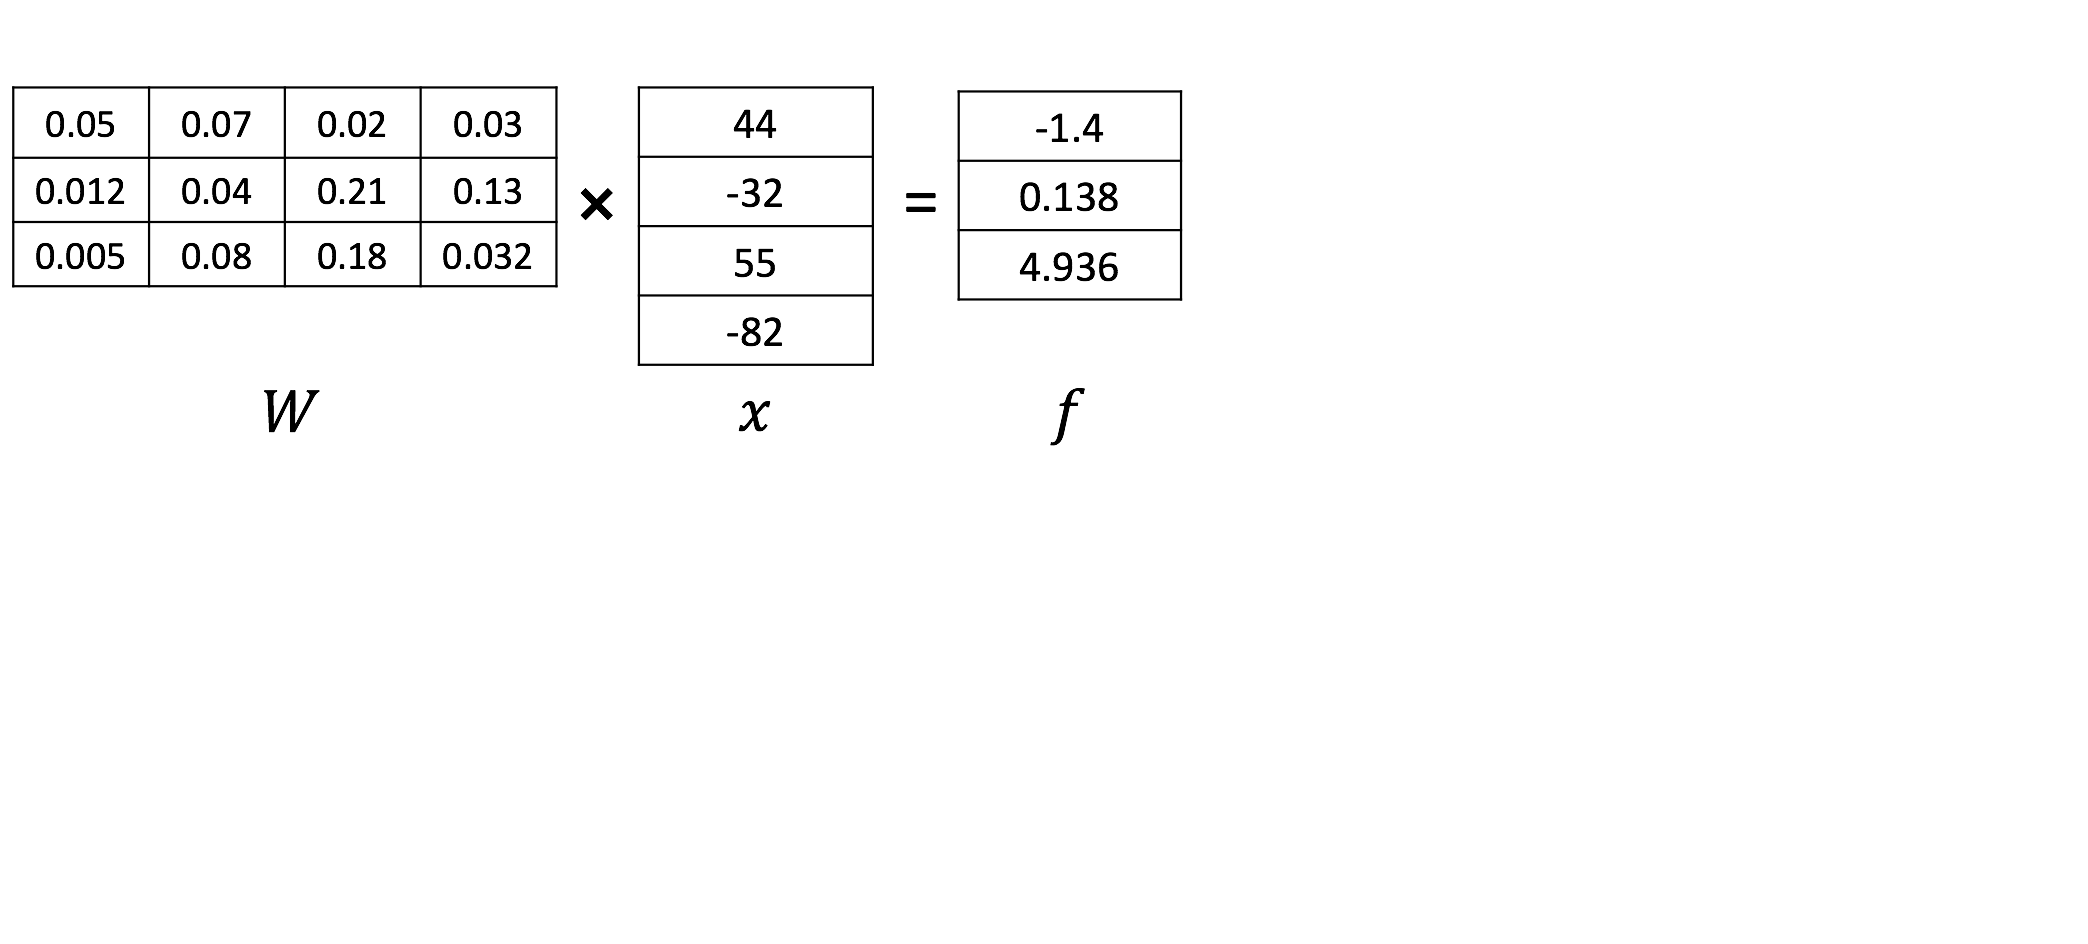
\includegraphics[width=1.05\textwidth]{softmax_example2}
\end{center}
\end{frame}


\begin{frame}{Softmax Cost Function Example}
\begin{center}
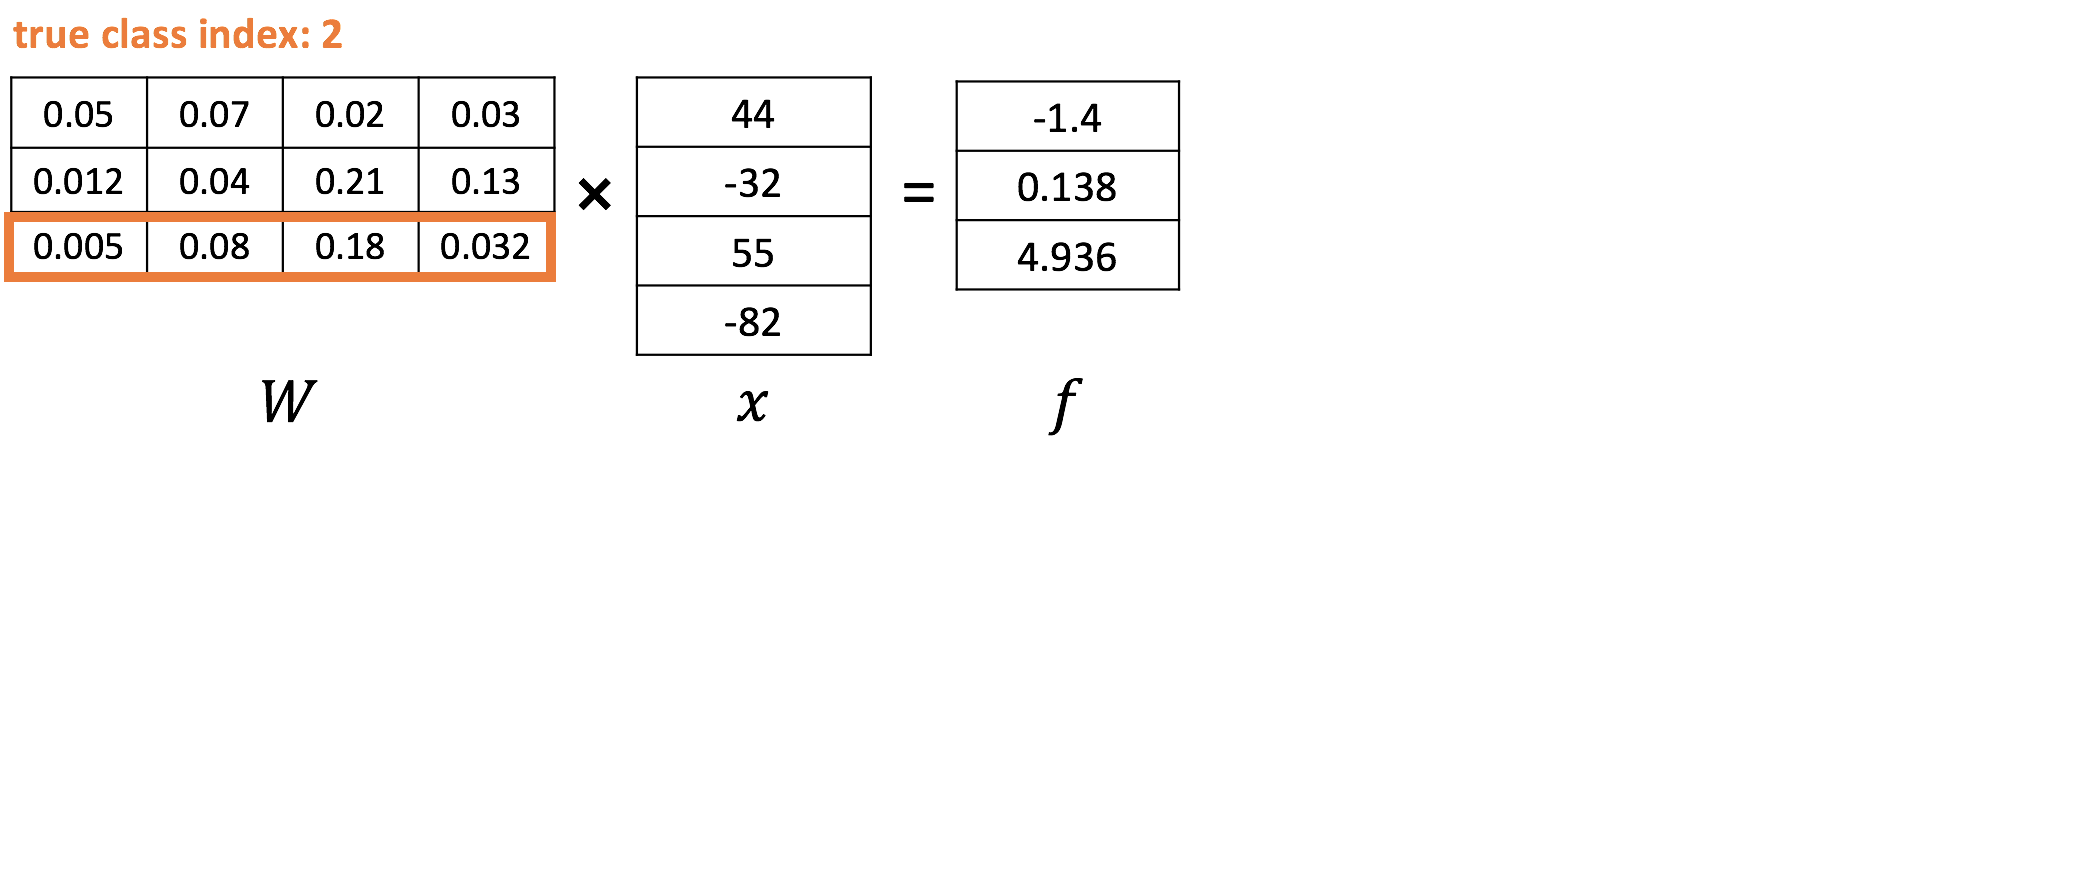
\includegraphics[width=1.05\textwidth]{softmax_example3}
\end{center}
\end{frame}

\begin{frame}{Softmax Cost Function Example}
\begin{center}
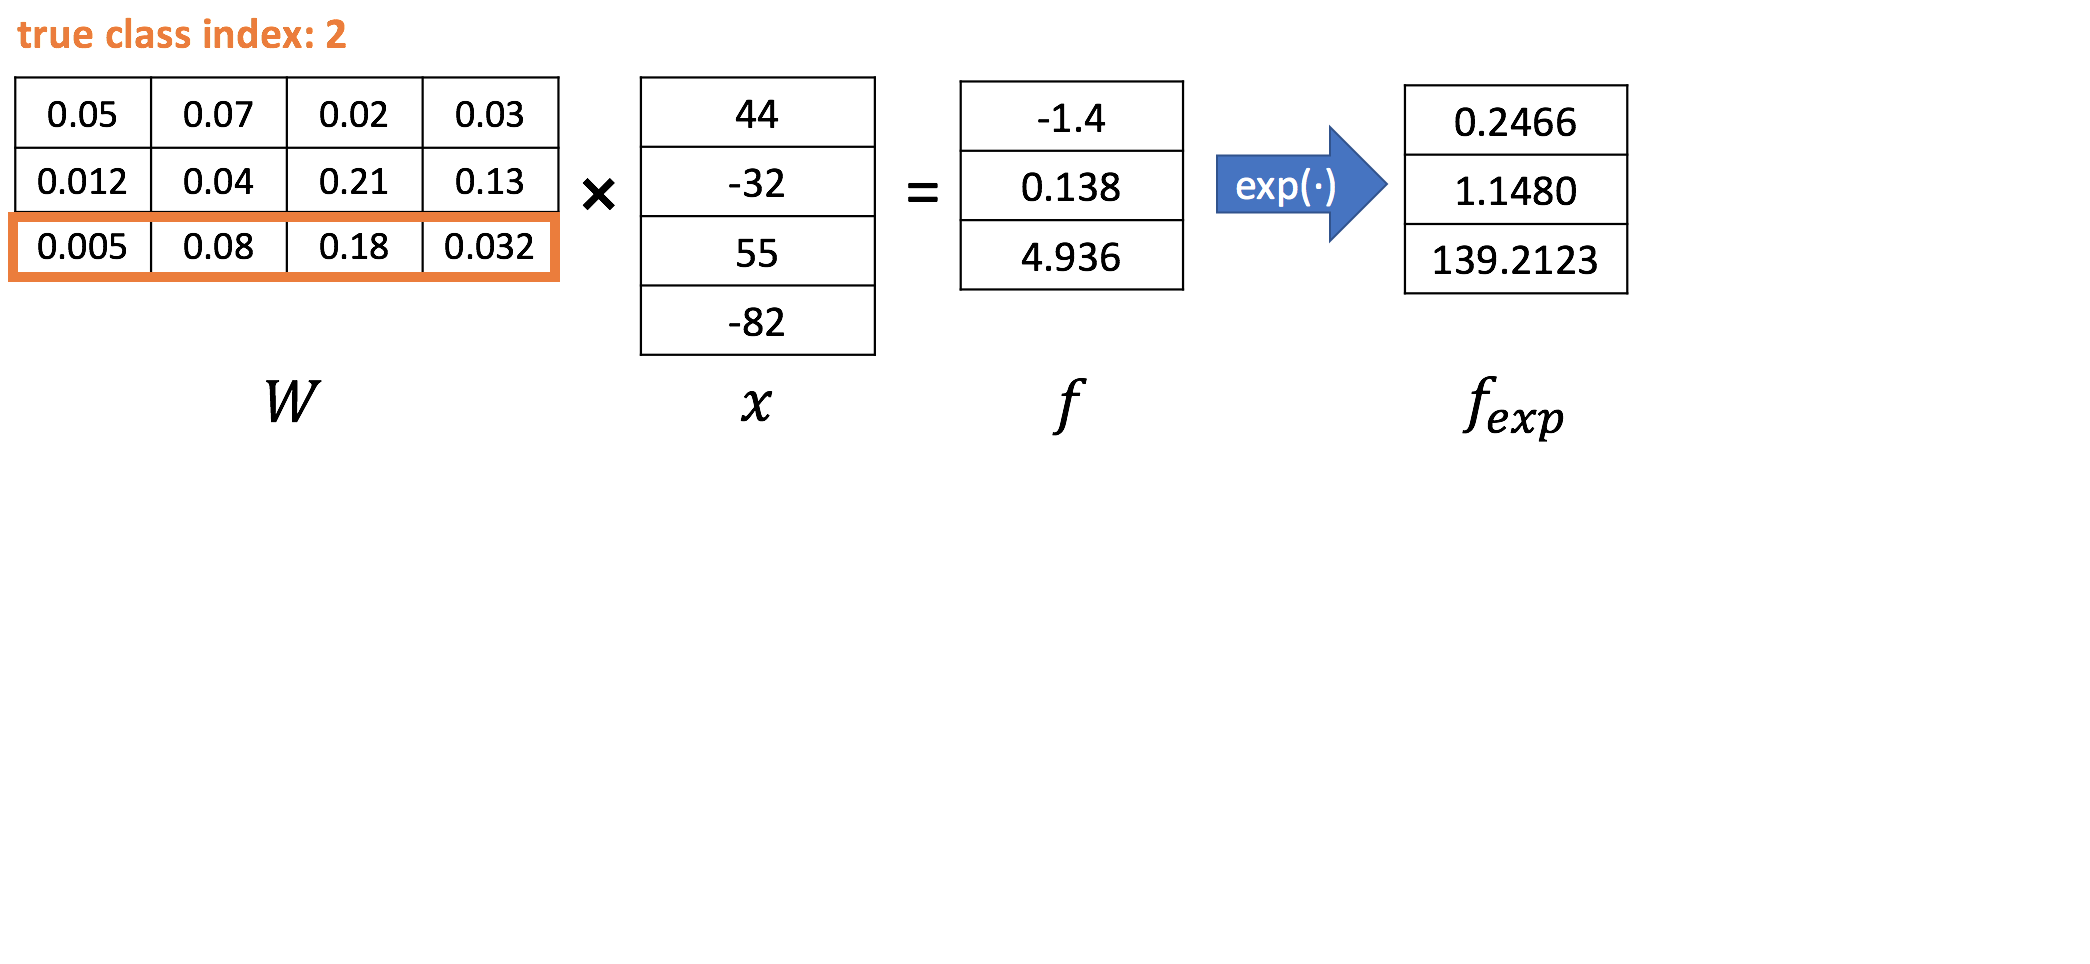
\includegraphics[width=1.05\textwidth]{softmax_example4}
\end{center}
\end{frame}


\begin{frame}{Softmax Cost Function Example}
\begin{center}
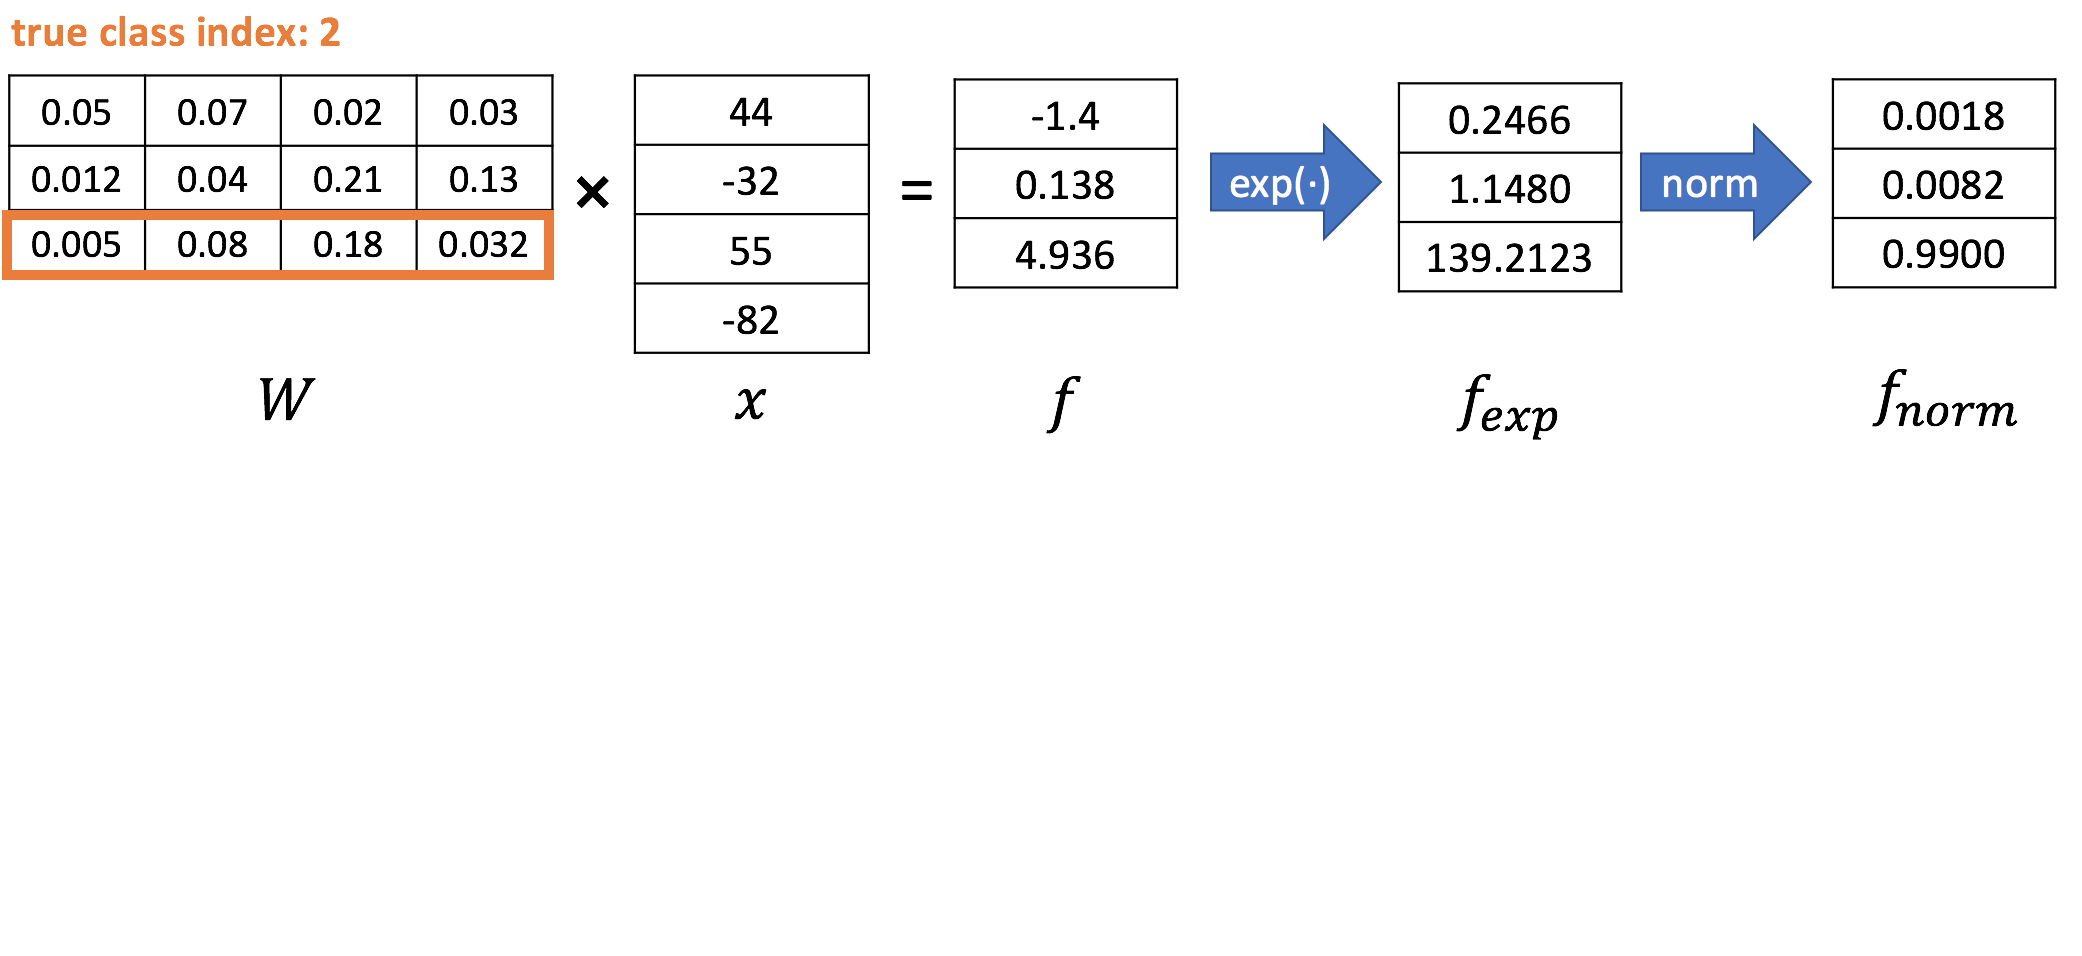
\includegraphics[width=1.05\textwidth]{softmax_example5}
\end{center}
\end{frame}

\begin{frame}{Softmax Cost Function Example}
\begin{center}
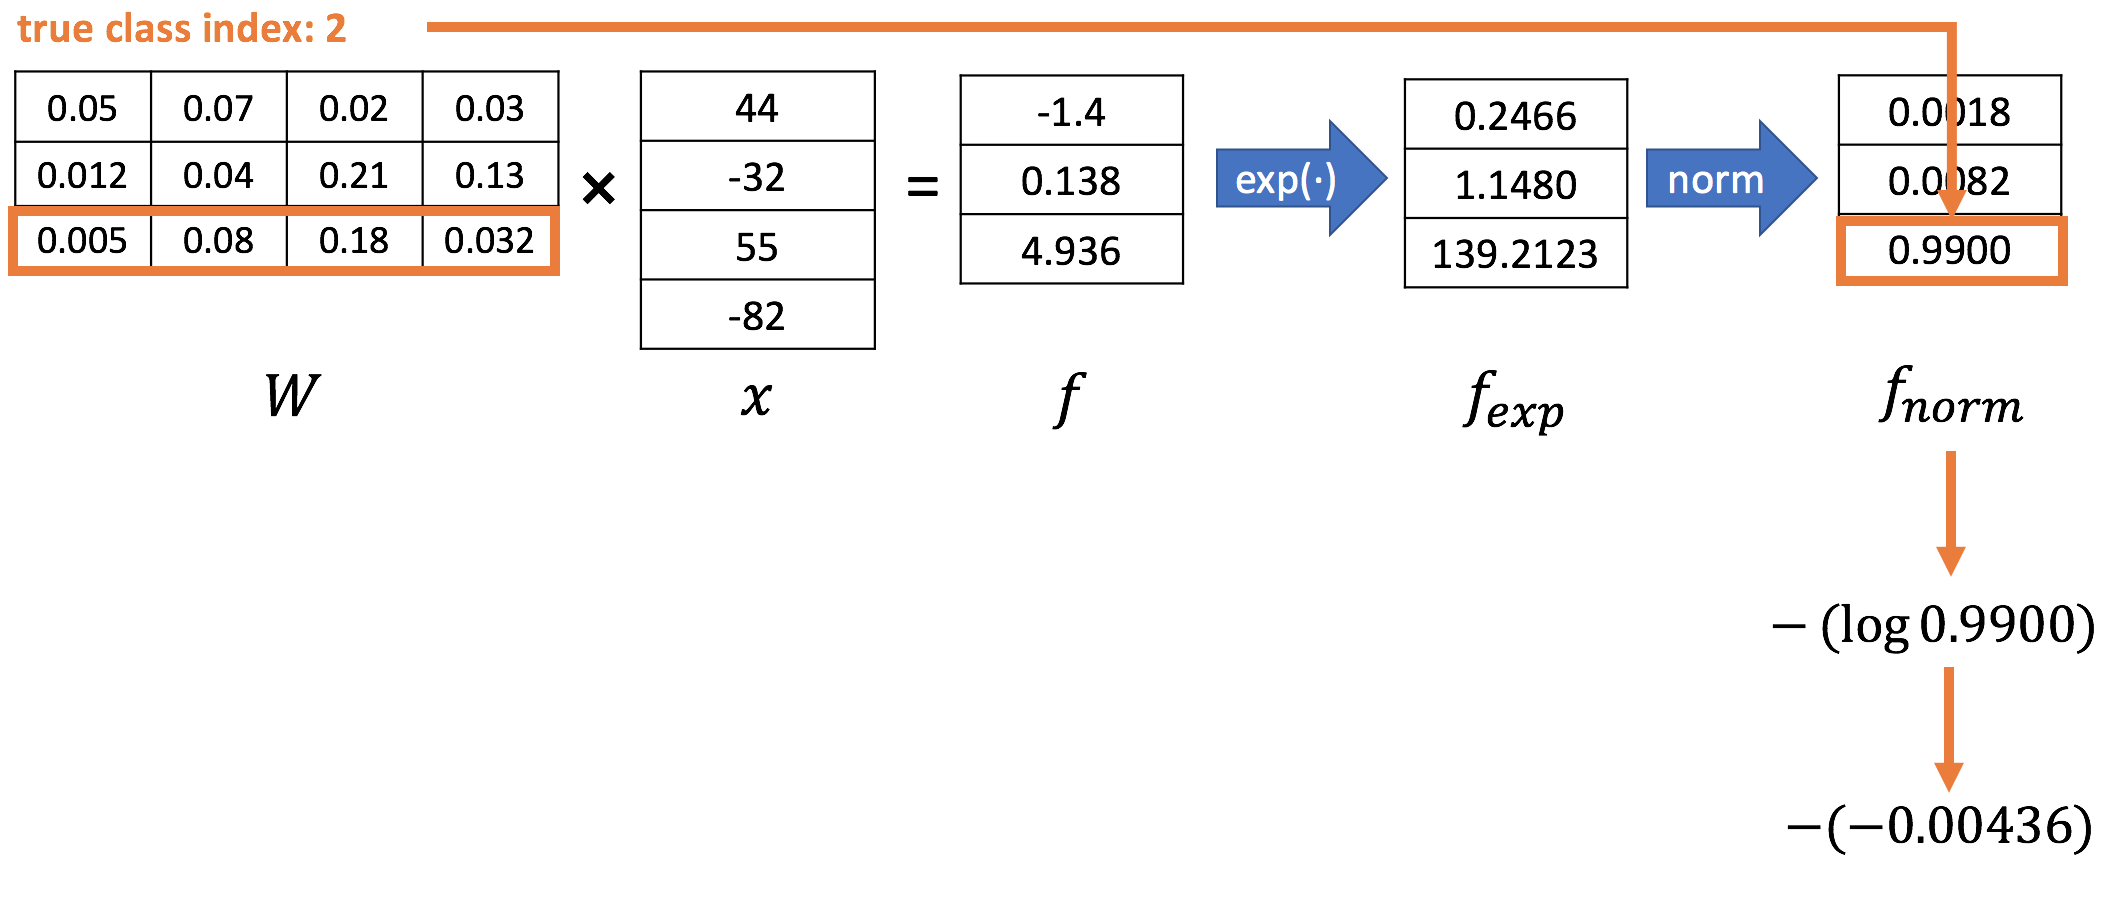
\includegraphics[width=1.05\textwidth]{softmax_example6}
\end{center}
\end{frame}

\begin{frame}{Backpropagation Algorithm}

\begin{itemize}
\item motivation: the cost function is in most cases non-linearly dependent on the parameters of a multi-layer NN\\
$\Rightarrow$ computing closed-form solution intractable or not possible
\item backpropagation executes two steps iteratively:
\begin{enumerate}
\item forward-pass: computes the loss $L_i$ and its gradient 
\item backward-pass: updates $W$ with gradient descent $\Rightarrow$ minimizes $L_i$ iteratively \footnote{repeatedly applying gradient descent within backprop is sometimes called \emph{stochastic gradient descent}, \emph{stochastic} here usually refers to "on-line"}
\end{enumerate} 
\end{itemize}
\end{frame}

\begin{frame}{Backpropagration Algorithm}
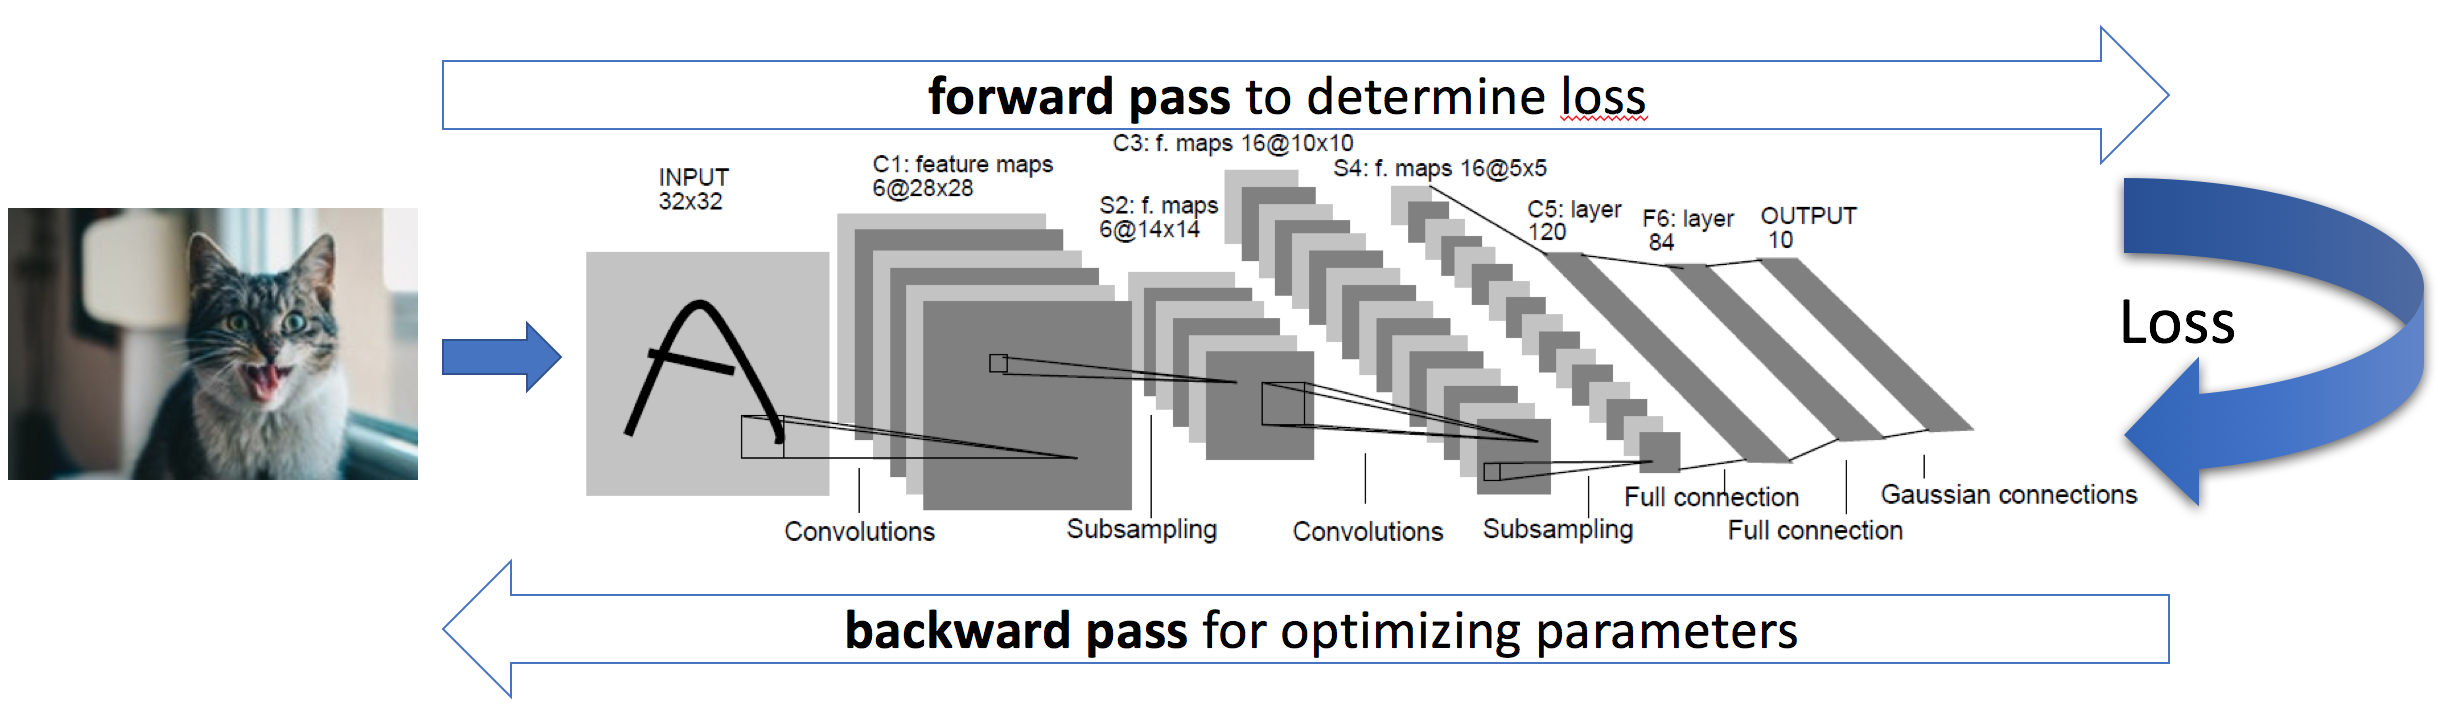
\includegraphics[width=1.1\textwidth]{backprop}\\

source: Yann LeCun et al., „Gradient-Based Learning Applied to Document Recognition“
\end{frame}

\begin{frame}{Connection between Backprop and Learning Theory class}
\textbf{Q}: What is the solver actually doing when executing the backpropagation algorithm?\\
\uncover<2->{\textbf{A}:it executes a search within the hypothesis space for a suitable hypothesis (remember hypothesis space theory class)\\}
\uncover<3->{\textbf{Q}: What are the hypotheses?\\}
\uncover<4->{\textbf{A:} the individual weight vector per iteration (relative to the training examples)\footnote<4->{this also holds for weight vectors in Logistic Regression computed by Gradient Descent methods}. More precisely: the hypothesis space contains \textbf{continuously} parameterized hypotheses (for example the weights in the neurons)}\\
\uncover<5->{The \textbf{inductive bias} by which backprop generalizes beyond seen data is a bit more tricky: it's the smooth interpolation between data points (i.e. labels between two positive samples will also be positive}
\end{frame}

%decision tree hypothesis search is discrete

\begin{frame}{Backpropagation Algorithm: the Backward Pass}
\begin{itemize}
\item To update the weights, Backpropagation computes the direction of the steepest descent in the $n$-dimensional space:
\begin{equation}
	\nabla L(W) = \frac{\partial L}{\partial w_0}, \frac{\partial L}{\partial w_1}, ..., \frac{\partial L}{\partial w_n}
\end{equation}
\item We use the following (or a more sophisticated) rule to update the weights of every single neuron\footnote{called vanilla update}:
\begin{equation}
w_{t+1} = w_t + v_{t+1}
\end{equation} 
\begin{equation}
v_{t+1} = - \alpha \frac{\partial L}{\partial w_t}
\end{equation}
with $w_t$ being the parameter vector at time step $t$ and $\alpha$ the learning rate
\end{itemize}
\end{frame}

\begin{frame}{Backpropagation Algorithm: the Backward Pass}
\begin{itemize}
\uncover<1->{\item computing the gradients between the output and the last hidden layer is straightforward (derive loss fct. w.r.t. to the individual weight)}
\uncover<2->{\item the gradients of $L$ w.r.t to the weights $w_{j,i}$ (weight between neuron i to j) previous to the last hidden layers are \textbf{unknown} at first}
\uncover<3->{\item solution: we use the \textbf{chain rule} to compute the gradients between the last and penultimate layer, the penultimate and the layer previous to that etc.
\begin{equation}
	 \frac{\partial L}{\partial w_{j,i}} = \frac{\partial L}{\partial z_j} \times \frac{\partial z_j}{\partial w_{j,i}}
\end{equation}}

with $z_j$ being the output of neuron $j$ 
\end{itemize}
\end{frame}

\begin{frame}{Backpropagation Algorithm: the Backward Pass}
\begin{center}
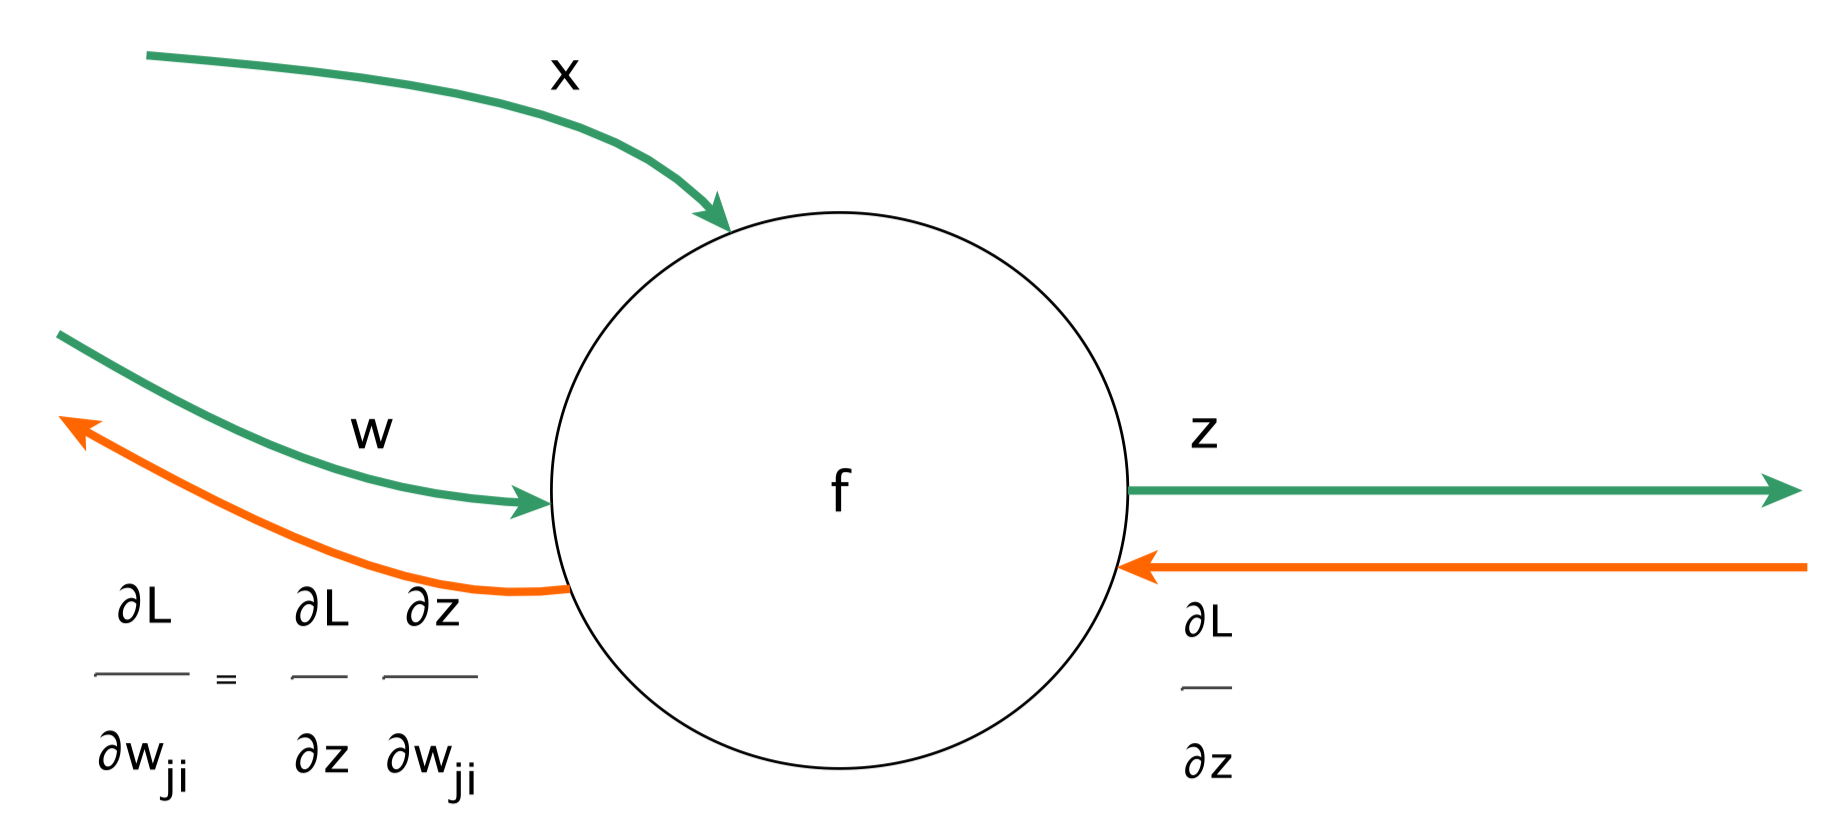
\includegraphics[width=1\textwidth]{backprop2}
\end{center}
lecture recommendation for backprop and chain rule (Stanford's CS231n course)\footnote{\url{https://www.youtube.com/watch?v=i94OvYb6noo&t=322s}}
\end{frame}


\begin{frame}{Extensions to Learning NN and Problems}

\begin{itemize}
\item the weight update rule is often subject to change since it tends to get stuck in local minima
\item exemplary extension; momentum update:
\begin{equation}
v_{t+1} = - \alpha \frac{\partial L}{\partial w_t} + \mu v_t
\end{equation} $\mu \in [0,1]$

\item initialization of weights matter (see next slide)\\
$\Rightarrow$ \textbf{vanishing gradient} and \textbf{exploding gradient problem}
\item use initialization methods, e.g. \emph{Xavier} initialization
\item \textbf{saturating activation functions} can cause problems as well
\item small/large learning rates $\Rightarrow$ common: adaptive /decreasing LR
\end{itemize}
\end{frame}

\begin{frame}{Vanishing Gradients}
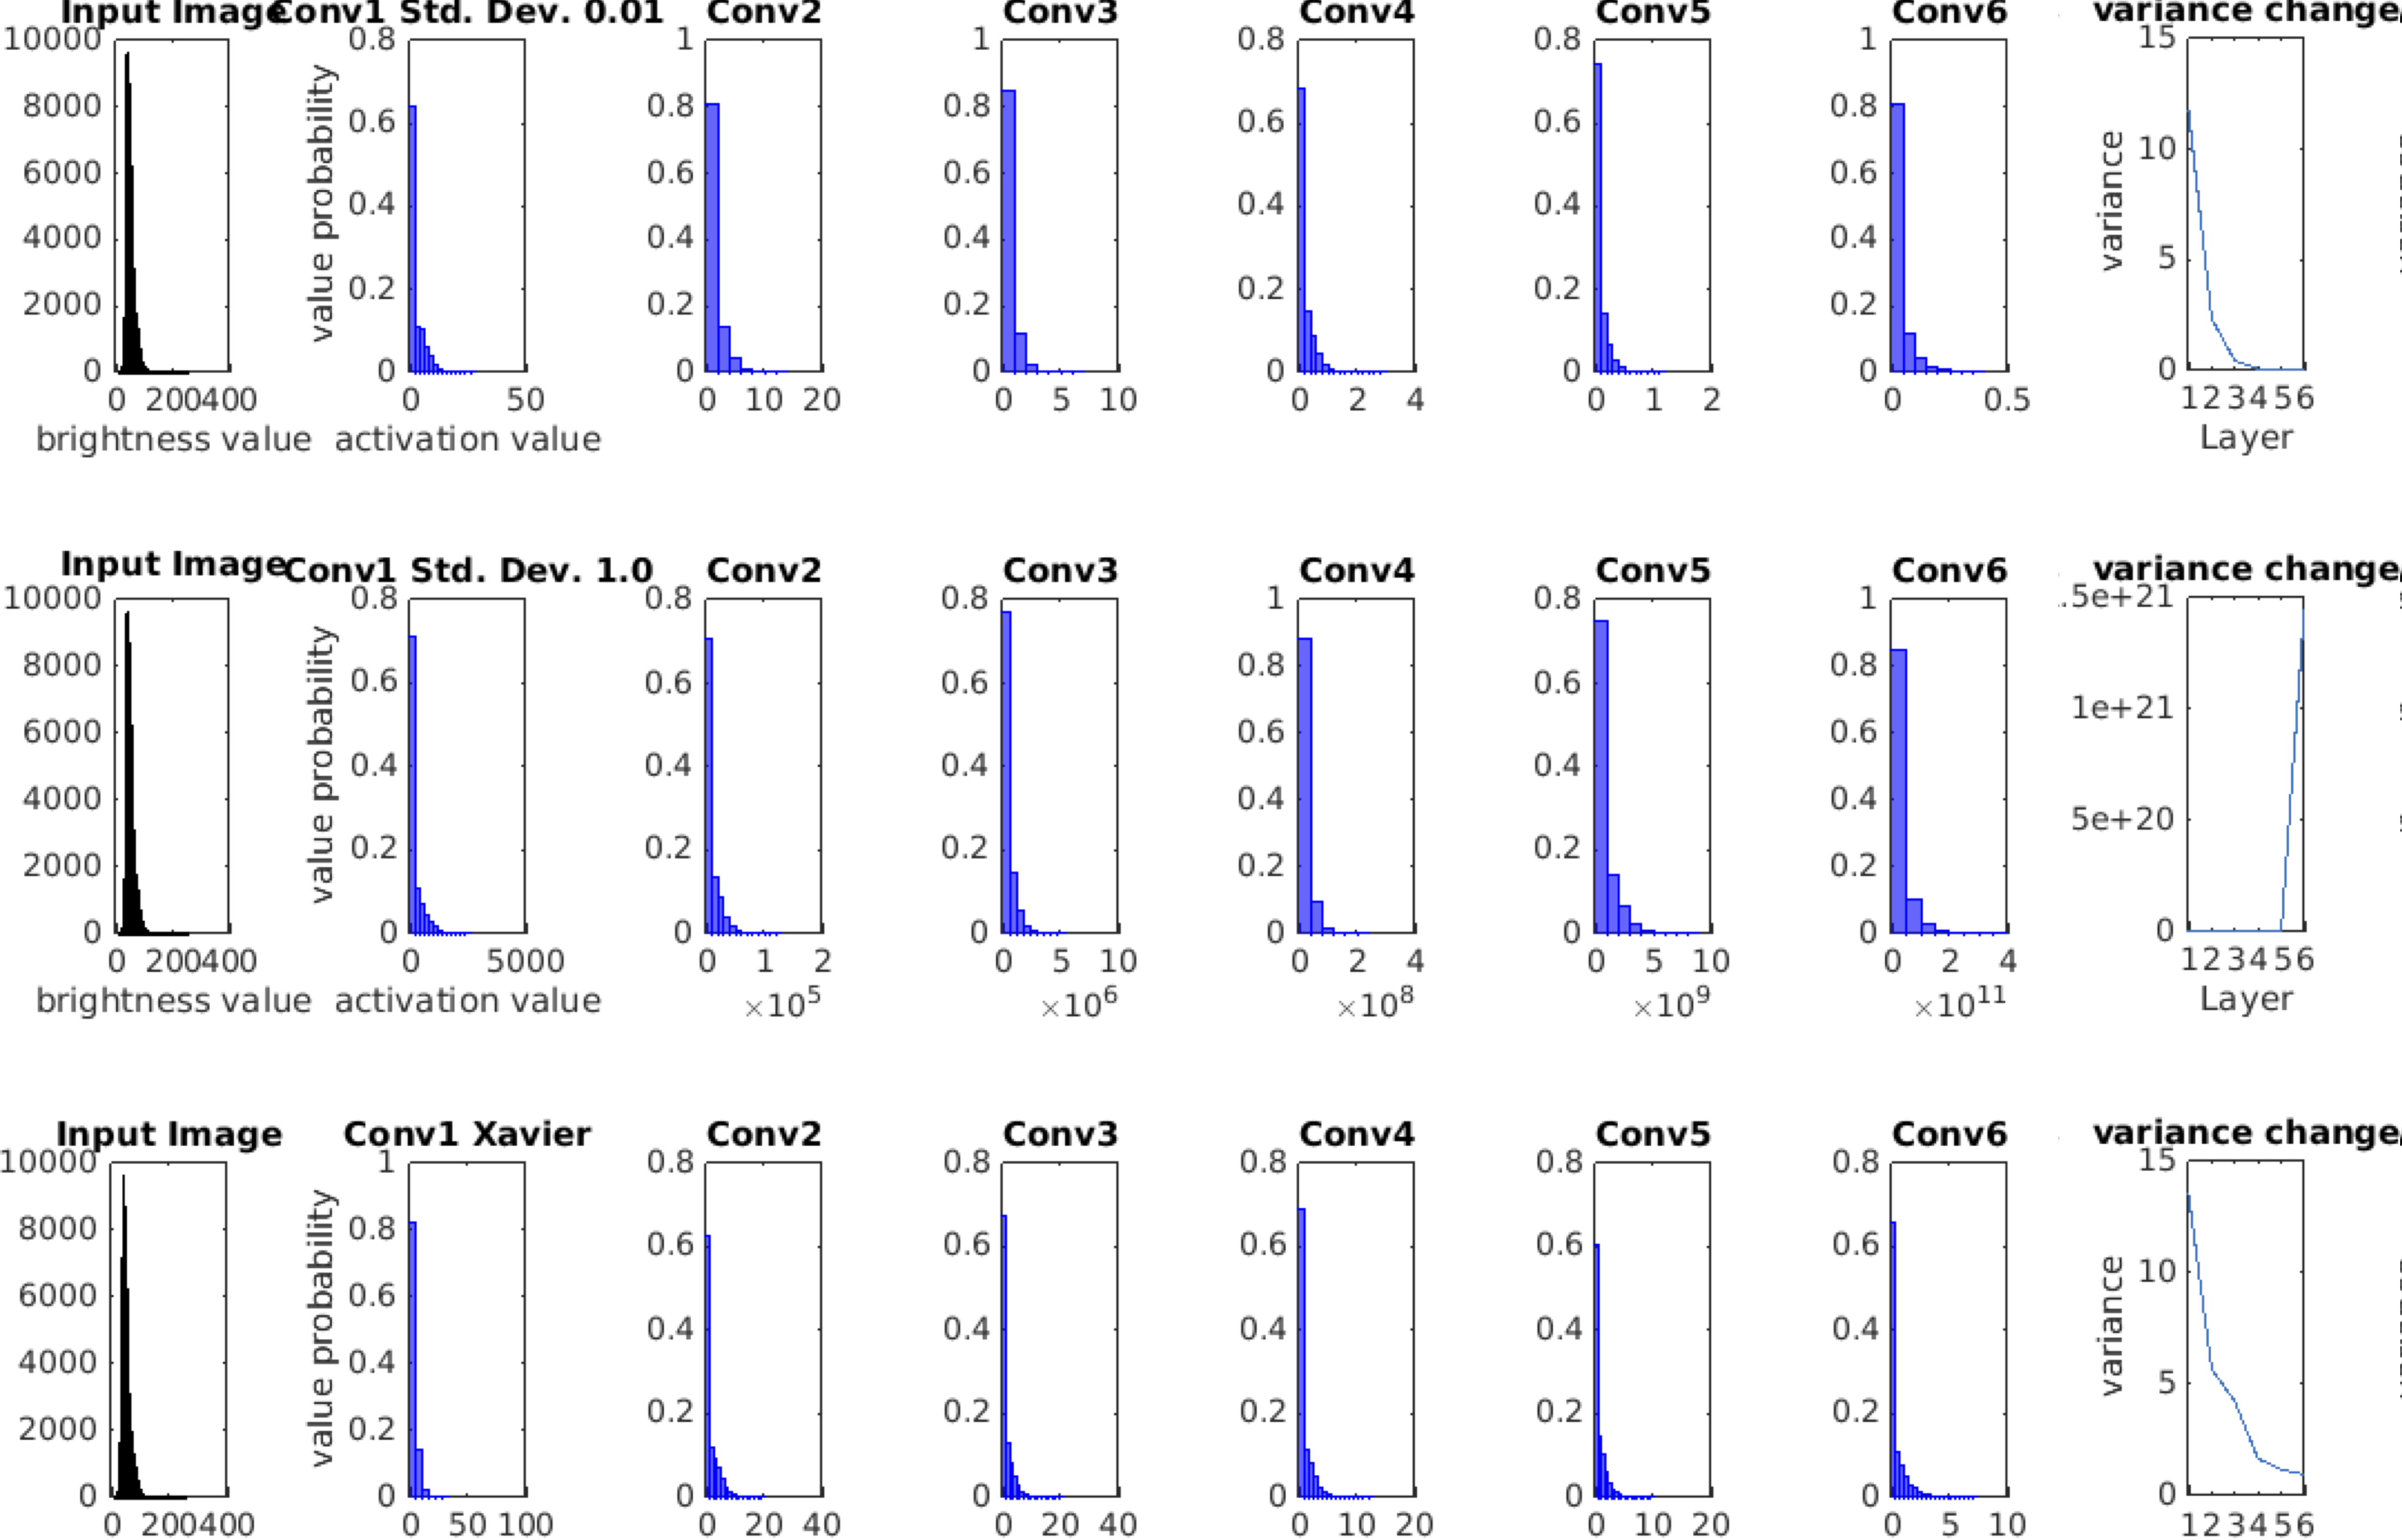
\includegraphics[width=1\textwidth]{vanishing}
\end{frame}


\begin{frame}{Regularization}
\begin{itemize}
\item \textbf{regularization} is a collective term for methods that reduce overfitting
\item regularization through a \textbf{penalty term} $R(W)$ (weight decay):
\begin{equation}
 L = \sum_i L_i + \lambda R(W)
\end{equation}

\begin{itemize}
\item L1: $R(W) = \lambda \sum_w |w|$
\item L2: $R(W) = \lambda \sum_w |w|^2$
\item typically $\lambda < 0.1$
\end{itemize}
\item L1 allows concentrations within weight distributions (focus on some features)
\item L2 penalizes outliers more strongly, fewer concentrations (focus on all features)
\end{itemize}
\end{frame}


\begin{frame}{Regularization}
\begin{itemize}
\item R(W) enforces a NN to have small weights\\
$\Rightarrow$ have many small weights instead of few big weights (more inputs considered)
\end{itemize}
further regularization techniques:
\begin{itemize}
\item \textbf{dropout}: remove dependencies among neurons
\item \textbf{data augmentation}: enlarge small datasets
\item \textbf{architecture size}: decrease number of parameters to reduce risk of learning irrelevant features 
\end{itemize}
\end{frame}

\begin{frame}{Training and Testing Phases}
Training a NN gives rise to one particular question: when are we done with training? Best practice is: 
\begin{itemize}
\item have a train / valid and test split of your data
\item typically do validation phase after $n$ training iterations
\item plot or print train and valid loss\footnote{or accuracy, prediction, recall, f-score etc.}
\item both losses shouldn't diverge (overfitting)
\end{itemize}
\end{frame}

\begin{frame}{Training and Testing Phases}
Optimal stopping problem: don't stop too early but also not too late 
\begin{center}
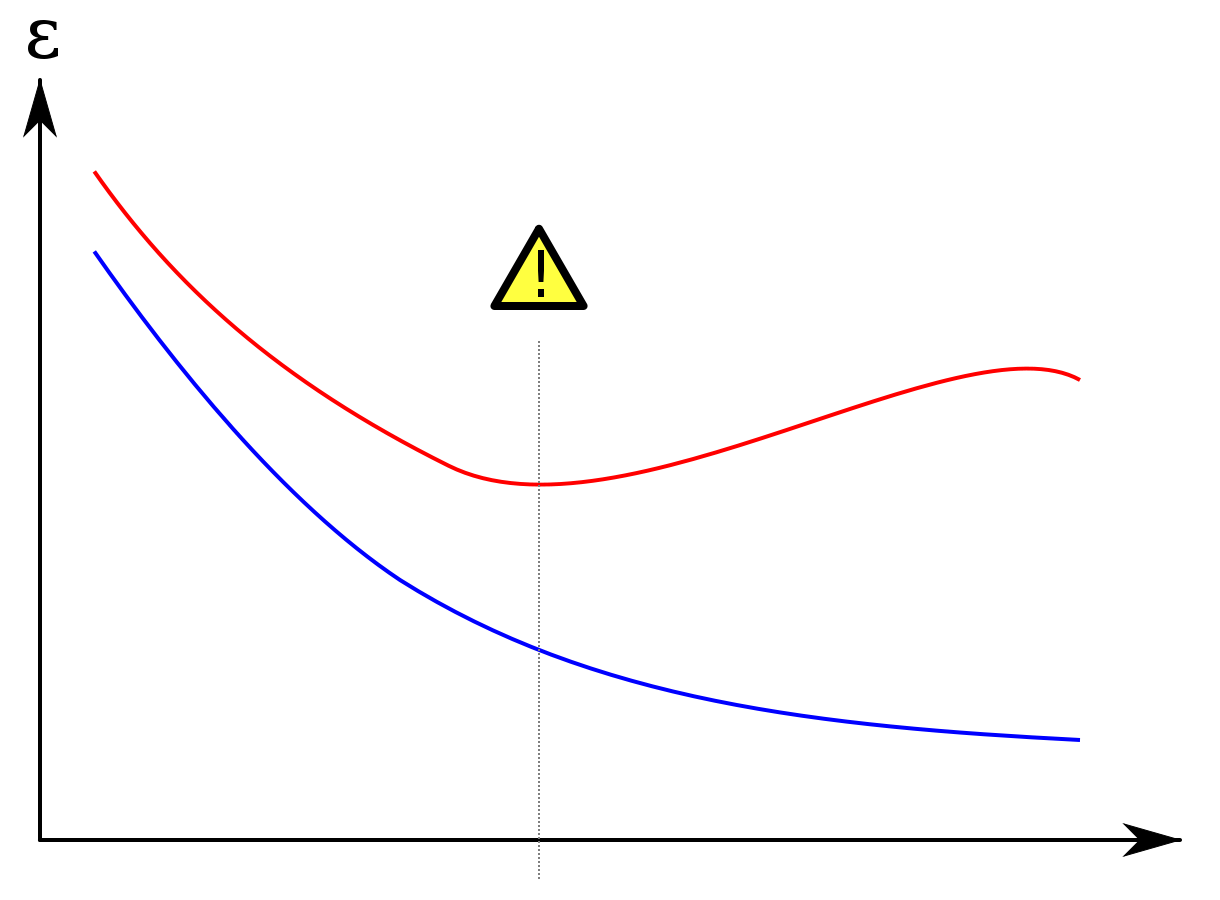
\includegraphics[width=0.7\textwidth]{overfitting_nn}\\
(blue: training loss, red: validation loss)
\cite{WikiOverfitting}
\end{center}
\end{frame}

\subsection{NNs for Perception: Convolutional Neural Networks}
\begin{frame}{Convolutional Neural Networks}
\begin{itemize}
\uncover<1->{\item CNN's are a variant of multi-layer NN}
\uncover<2->{\item their design is inspired by biological processes\\$\Rightarrow$ neurons in the animal visual cortex respond to stimuli only in a restricted area}
\uncover<3->{\item main difference to NN: neurons are not fully connected to underlying and overlying neighbor neurons\\$\Rightarrow$ "receptive field"\\
\begin{center}
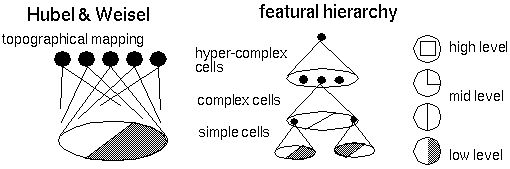
\includegraphics[width=0.6\textwidth]{hubel_wiesel}
\cite{T.N.Wiesel1959}
\end{center}}
\end{itemize}
\end{frame}

\begin{frame}{Convolutional Neural Networks}
typically use three types of layers
\begin{itemize}
\item convolutional layer (conv layer)
\item pooling layer
\item fully-connected layer (fc layer)
\end{itemize}

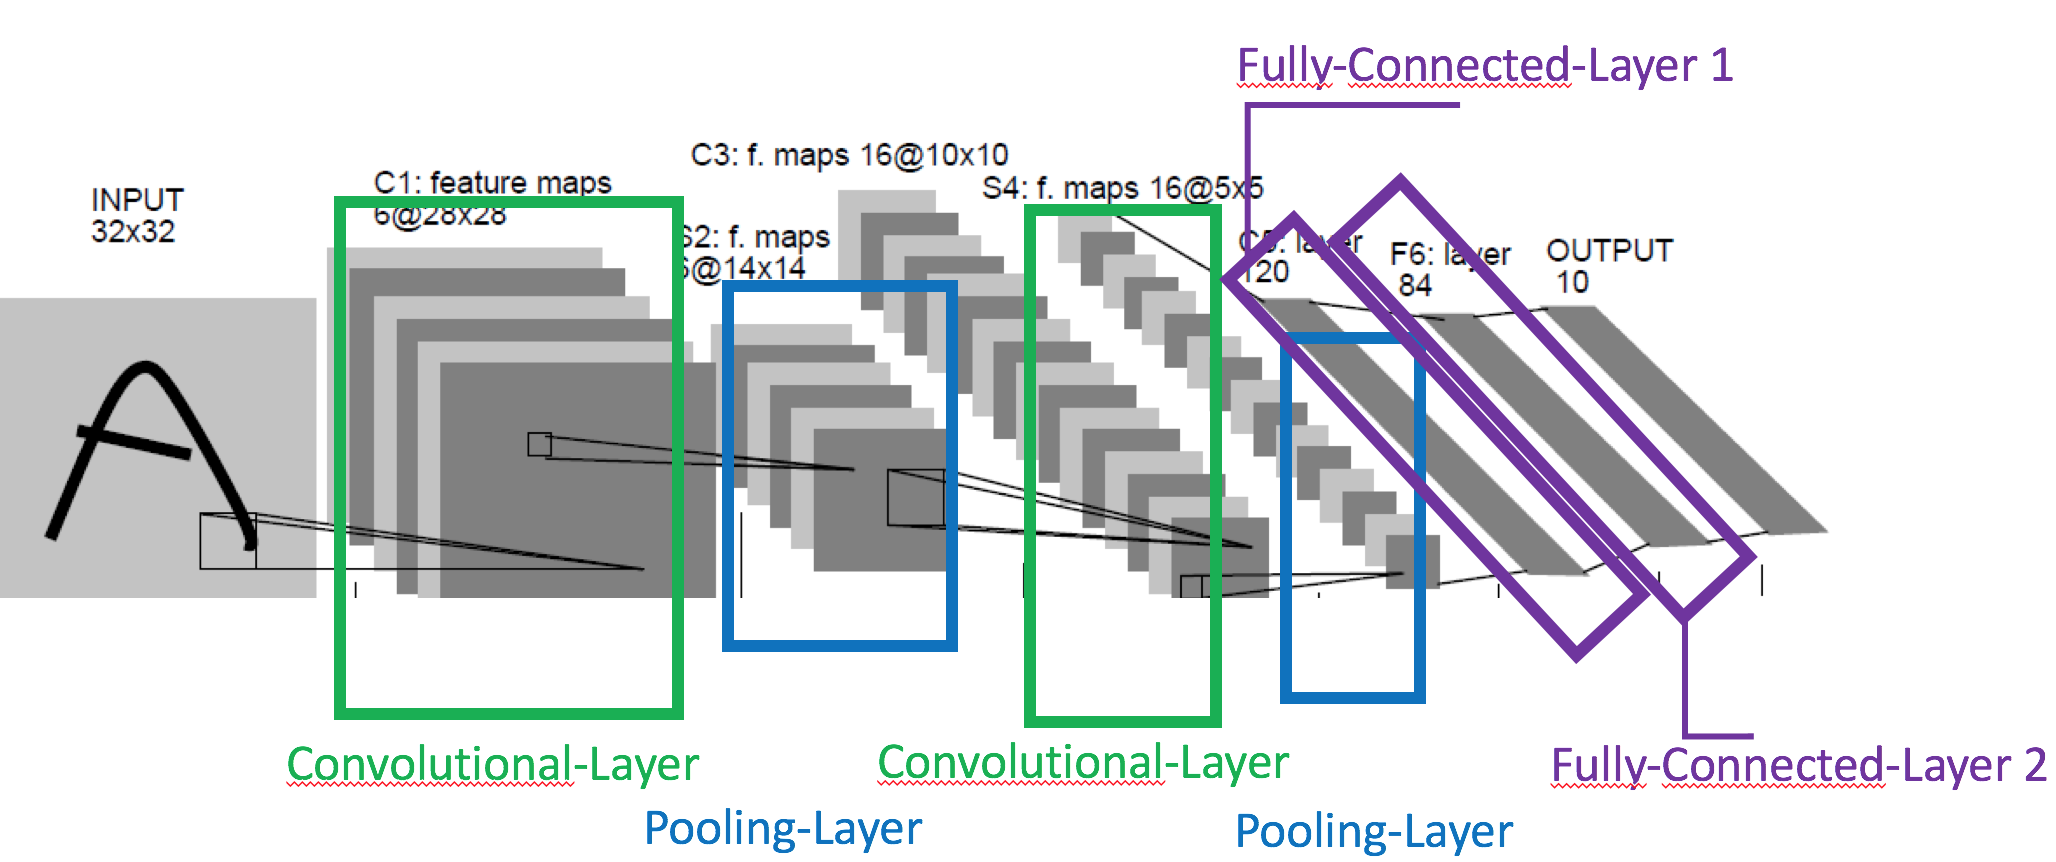
\includegraphics[width=0.9\textwidth]{lenet2}
\end{frame}

\begin{frame}{CNN's: Convolutional Layer}
\begin{center}
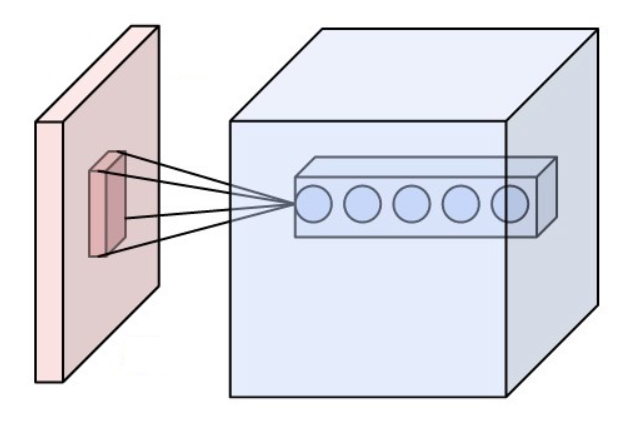
\includegraphics[width=0.5\textwidth]{conv_layer}\\
\cite{ConvWiki}
\end{center}

\begin{itemize}
\uncover<1->{\item receptive field is slided over the input}
\uncover<2->{\item the parameters learned in a conv layer are the elements of the filter matrices}
\uncover<3->{\item depth of the "block" is defined by the number of filters}
\uncover<4->{\item detects e.g. edges, circles, cat ears etc.}
\end{itemize}
\end{frame}

\begin{frame}{CNN's: Pooling Layer}
\begin{center}
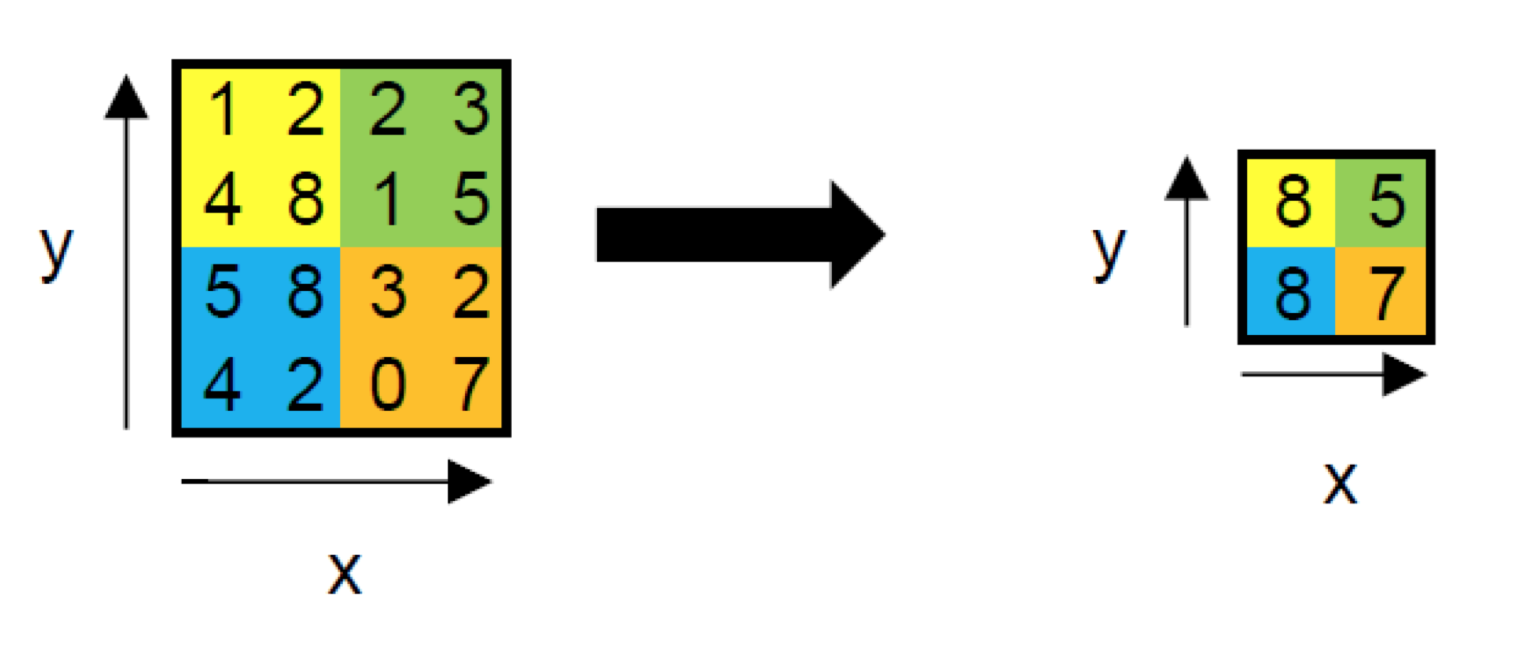
\includegraphics[width=0.7\textwidth]{pooling}
\end{center}
\begin{itemize}
\uncover<1->{\item reduces the number of learned parameters}
\uncover<2->{\item achieves invariance to small translations in the input / features}
\uncover<3->{\item maximum and average pooling most common}
\end{itemize}
\end{frame}

\begin{frame}{CNN's: features visualized}
\begin{center}
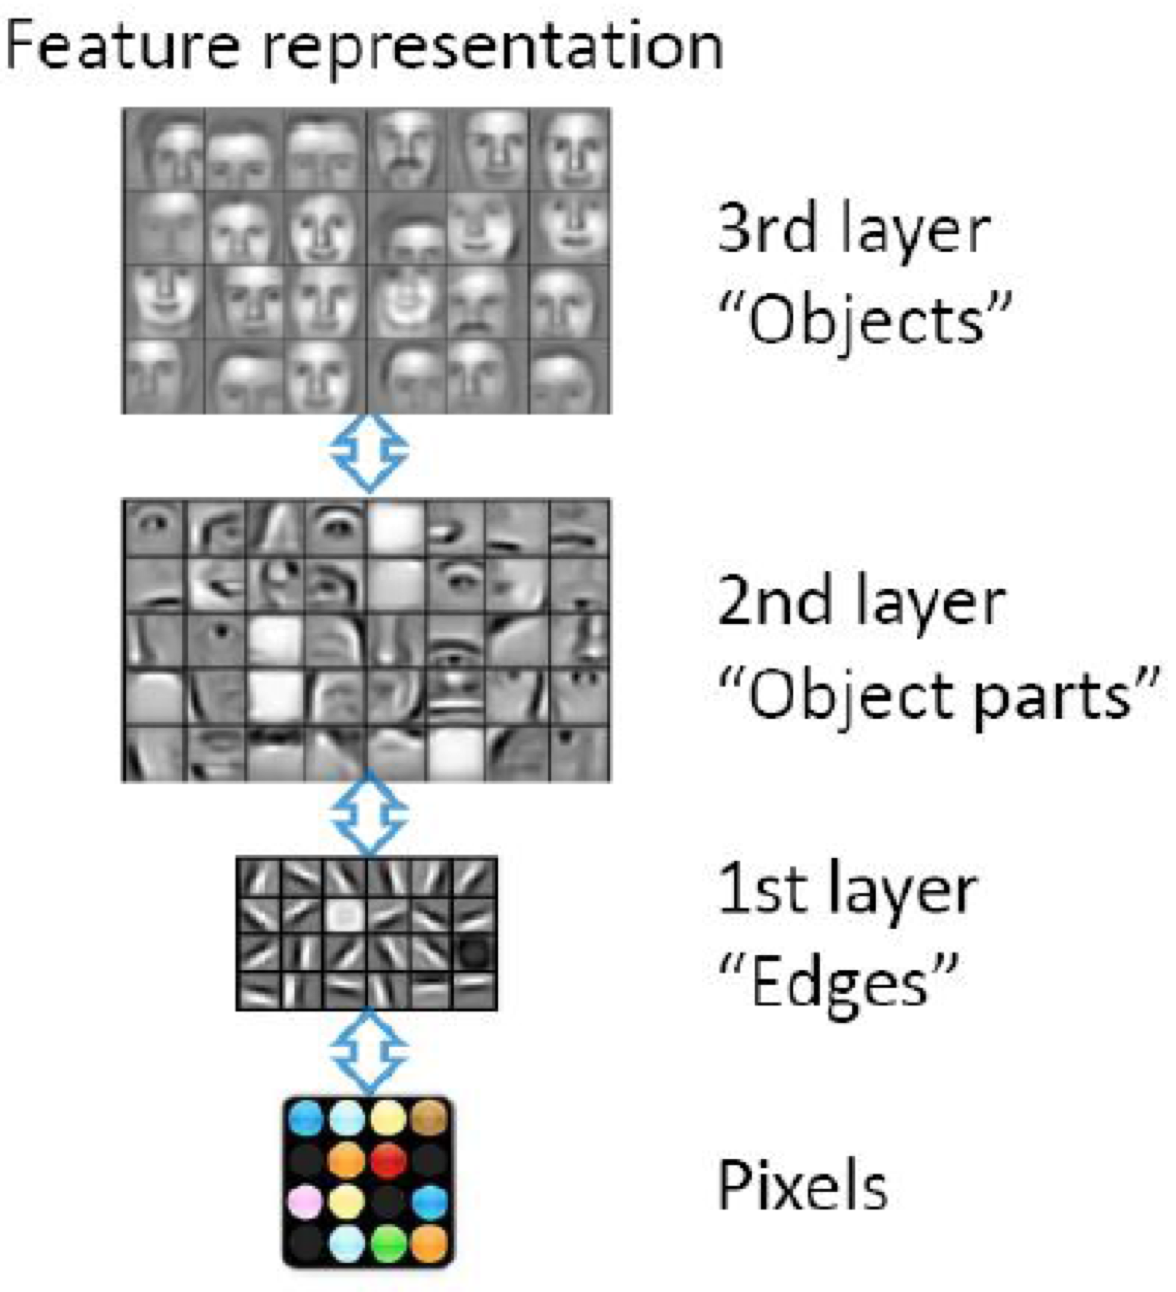
\includegraphics[width=0.5\textwidth]{cnn_features}\\
source: Honglak Lee, “Tutorial on deep learning and applications”
\end{center}
\end{frame}

\subsection{Words of Advice}


\begin{frame}{Some Advices for Practical Applications}
\begin{itemize}
\uncover<1->{\item invest in data-preprocessing, data normalization}
\uncover<2->{\item use a healthy dataset split, e.g. 70/20/10 (train/valid/test)}
\uncover<3->{\item a good optimizer (solver) is "Adam" (per-parameter LR \& moving averages of the gradient)}
\uncover<4->{\item use ReLU, PReLU etc.}
\uncover<5->{\item careful with bounded activation functions (e.g. sigmoid in regression) in the output layer}
\uncover<6->{\item 64 or 128 filters for conv layers is plenty}
\uncover<7->{\item currently popular frameworks: PyTorch, TensorFlow}
\uncover<8->{\item training on GPUs is generally faster than training on CPUs}
\uncover<9->{\item try to get a feeling for depth and breadth of NNs/CNNs with the ConvNetJS demo: \url{https://cs.stanford.edu/people/karpathy/convnetjs/demo/classify2d.html}}
\end{itemize}
\end{frame}

\begin{frame}{When not to use Deep Neural Networks}
Deep Learning is not the answer to everything; sometimes simpler models work 
better. When should you not use it?
\begin{itemize}
\item if you don't have enough data
\item if it's a low budged project (DL requires many resources such as GPUs,  time for training and paper research etc.)
\item when traceability is important or when causal mechanisms need to be understood (although research is slowly getting there)
\end{itemize}
\end{frame}


\subsection{Exercise: Training a Classifier}

\begin{frame}{Application: Training a Classifier}
IMO: best way of learning is to experiment around. Therefore, I suggest to try the following tutorial as a voluntary homework:
\begin{itemize}
\item \url{http://pytorch.org/tutorials/beginner/blitz/cifar10_tutorial.html}
\item training of an image classifier with a CNN
\item Python novice skills are sufficient
\item no GPU required (before downloading, choose "CUDA: None")
\item requires PyTorch (mac OS, Linux, Windows)
\item uses CIFAR10 dataset; 60 000 32x32 color images of 10 classes
\item we can discuss issues either on Moodle or during the upcoming lectures
\end{itemize}
\end{frame}

\subsection{CNN Applications}
\begin{frame}{Neural Networks in Practice}
\begin{itemize}
\item CNNs for face recognition [Taigman et al., 2014, "DeepFace"]
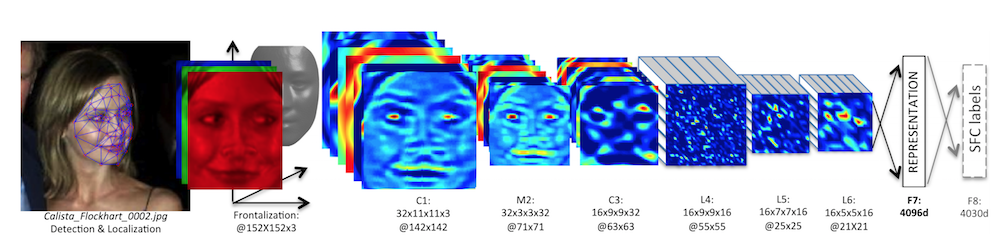
\includegraphics[width=0.7\textwidth]{cnn_app1}
\item CNNs for human pose estimation [Toshev et al., 2014]\\
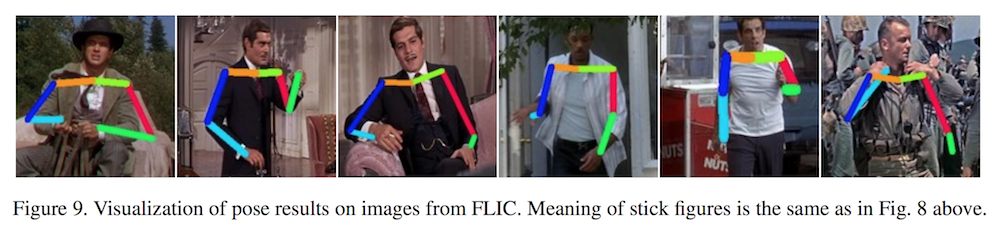
\includegraphics[width=0.7\textwidth]{cnn_app2}
\end{itemize}
\end{frame}


\begin{frame}{Neural Networks in Practice}
\begin{itemize}
\item CNNs for style transfer [Gatys et al., 2015, "DeepArt"]
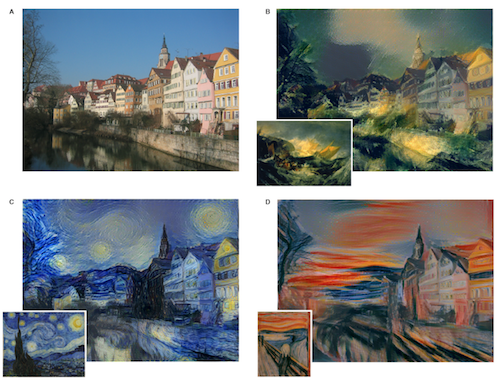
\includegraphics[width=0.4\textwidth]{cnn_app4}
\item CNNs used in GANs [Karras et al., 2018]\\
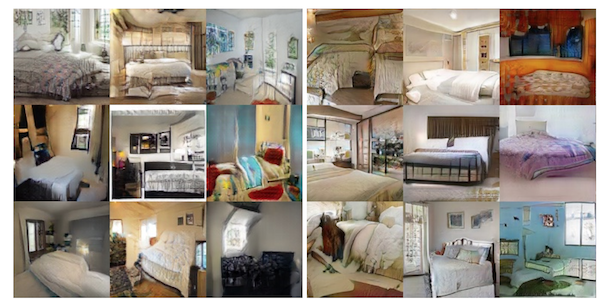
\includegraphics[width=0.5\textwidth]{cnn_app5}
\end{itemize}
\end{frame}




\newpage
\bibliographystyle{apalike}
\bibliography{lecture/bibliography.bib}

\end{document}
